\documentclass[a4paper,12pt]{report}

% Page layout
\usepackage[left=2.5cm,right=2.5cm,top=2.5cm,bottom=2.5cm]{geometry}

% Font and text
\usepackage[afrikaans,english]{babel}
\usepackage{microtype}
\usepackage{setspace}
\usepackage{lmodern}
\usepackage{siunitx}
\newcommand{\myemph}[1]{{\sffamily\bfseries#1}}
\sloppy
\onehalfspacing

% Headings
\usepackage[raggedright,sf,bf]{titlesec}
\usepackage[margin=\the\parindent,small,bf,sf]{caption}
\titlelabel{\thetitle.\ }
\titleformat{\chapter}[display]{\huge\bfseries\sffamily}{\chaptertitlename\ \thechapter}{15pt}{\Huge \raggedright}
\titlespacing*{\chapter}{0pt}{0pt}{40pt}  % remove spacing before chapter headings
\makeatletter
\let\originall@chapter\l@chapter
\def\l@chapter#1#2{\originall@chapter{{\sffamily #1}}{#2}}
\makeatother

%% Alternative headings using small-caps (comment out the top section)
%\usepackage[raggedright,bf]{titlesec}
%\usepackage[margin=\the\parindent,small,bf]{caption}
%\titlelabel{\thetitle.\ }
%\titleformat{\chapter}[display]{\huge\scshape}{\chaptertitlename\ \thechapter}{15pt}{\Huge \raggedright}
%\titlespacing*{\chapter}{0pt}{0pt}{40pt}  % remove spacing before chapter headings

% Table of contents
\let \savenumberline \numberline
\def \numberline#1{\savenumberline{#1.}}

% Figures
\usepackage{graphicx}
\usepackage{pdfpages}
\usepackage{float}
\usepackage{placeins}
\usepackage{subcaption}
\setlength{\abovecaptionskip}{7.5pt}  % spacing above and below captions
\newcommand*{\WaterMark}[2][0.2\paperwidth]{\AddToShipoutPicture*{\AtTextCenter{\parbox[c]{0pt}{\makebox[0pt][c]{\includegraphics[width=#1]{#2}}}}}}

% Mathematics
\usepackage[cmex10]{amsmath}
\usepackage{amssymb}
\usepackage{cancel}
\DeclareMathOperator*{\argmax}{arg\,max}
\newcommand{\T}{^\top}
\newcommand{\tr}{\textrm{tr}}
\renewcommand{\vec}[1]{\boldsymbol{\mathbf{#1}}}
\newcommand{\defeq}{\triangleq}

% Tables
\usepackage{booktabs}
\usepackage{tabularx}
\usepackage{multirow}
\newcommand{\mytable}{
    \centering
    \small
    \renewcommand{\arraystretch}{1.2}
    }
\renewcommand{\tabularxcolumn}[1]{m{#1}}
\newcolumntype{C}{>{\centering\arraybackslash}X}
\newcolumntype{L}{>{\raggedright\arraybackslash}X}

% Header and footer
\usepackage{fancyhdr}
\pagestyle{fancy}
\fancyhf{}
\renewcommand{\sectionmark}[1]{\markright{\normalsize \thesection.\ #1}}
\fancyhead[C]{\nouppercase{\textit{\rightmark}}}
\fancyhead[RO]{\thepage}
 \fancyhead[LE]{\thepage}  % double-sided printing
\fancyfoot{}
\setlength\headheight{14.5pt}
\renewcommand{\headrulewidth}{0pt}
\fancypagestyle{plain}{\fancyhead{}
                       \renewcommand{\headrulewidth}{0pt}
                       \fancyfoot[C]{\thepage}}

% Pseudo-code
\usepackage{algorithm}  % should go before \usepackage{hyperref}

% Table of contents and hyperlinks
\usepackage{hyperref}
\hypersetup{colorlinks=true,linktoc=all,citecolor=black,linkcolor=black}
\usepackage[nottoc]{tocbibind}

% Pseudo-code
\usepackage{algpseudocode}  % should go after \usepackage{hyperref}
\renewcommand{\thealgorithm}{\arabic{chapter}.\arabic{algorithm}} 
\captionsetup[algorithm]{labelfont={bf,sf},font=small,labelsep=colon}

% Bibliography
\usepackage{cite}  % automatically reorder inline citations
\bibliographystyle{IEEEtran}

% Fix titlesec issue
\usepackage{etoolbox}
\makeatletter
\patchcmd{\ttlh@hang}{\parindent\z@}{\parindent\z@\leavevmode}{}{}
\patchcmd{\ttlh@hang}{\noindent}{}{}{}
\makeatother

% Todo Notes:
\newcommand\todo[1]{\textcolor{red}{#1}}

% Custom text color marking for editing
\usepackage{xcolor}
\newcommand{\needscite}[1]{\textcolor{orange}{#1}}
\newcommand{\rephrase}[1]{\textcolor{brown}{#1}}
\newcommand{\trimdown}[1]{\textcolor{darkgray}{#1}}
\newcommand{\fillout}[1]{\textcolor{olive}{#1}}
\newcommand{\tooai}[1]{\textcolor{brown}{#1}}

% Acronyms
\usepackage{acro}
\acsetup{
    first-style = long-short,  % First use: device-under-test (DUT)
    list/display = used,        % Only show acronyms actually used in text
}

% Define acronyms
\DeclareAcronym{DUT}{
    short = DUT,
    long = device-under-test,
    short-plural = s,
    long-plural-form = devices-under-test,
}
\DeclareAcronym{EIS}{
    short = EIS,
    long = electrochemical impedance spectroscopy,
}
\DeclareAcronym{POC}{
    short = POC,
    long = point-of-care,
}
\DeclareAcronym{PCB}{
    short = PCB,
    long = printed circuit board,
    short-plural = s,
    long-plural = s
}
\DeclareAcronym{DSP}{
    short = DSP,
    long = digital signal processing,
}
\DeclareAcronym{DAC}{
    short = DAC,
    long = digital-to-analogue converter,
}
\DeclareAcronym{ADC}{
    short = ADC,
    long = analogue-to-digital converter,
}
\DeclareAcronym{TIA}{
    short = TIA,
    long = transimpedance amplifier,
}
\DeclareAcronym{PGA}{
    short = PGA,
    long = programmable gain amplifier,
}
\DeclareAcronym{LPF}{
    short = LPF,
    long = low-pass filter,
}
\DeclareAcronym{MCU}{
    short = MCU,
    long = microcontroller unit,
    short-plural = s,
    long-plural = s
}


\begin{document}

% Front matter
\graphicspath{{frontmatter/fig/}}
\pagenumbering{Alph}
\begin{titlepage}
	\begin{center}
		
		
\includegraphics[width=10cm]{USlogo-top}
		
		\vfill
		
		{\sffamily \bfseries \huge A Multiplexed Impedance Analyser for Biosensing Applications \par}
		
		\vfill
		
		{\large {\Large Karl Voigt} \\ 24867209 \par}
		
		\vfill
		
		\vfill
		
		{Report submitted in partial fulfilment of the requirements of the module \\
			Project (E) 448 for the degree Baccalaureus in Engineering in the Department of
			Electrical and Electronic Engineering at Stellenbosch University. \par}
		
		\vfill
		
		{\large {Supervisor}: Dr T.\ Ebrahim} %\\
		% Department of Electrical and Electronic Engineering \par}
		
		\vfill
		
		{\Large October 2025}
	\end{center}
\end{titlepage}

%\graphicspath{{frontmatter/fig/}}
\pagenumbering{Alph}

\begin{titlepage}
	\begin{center}
		
		%
\includegraphics[width=10cm]{USlogo-top}
		
		\WaterMark{UScrest-WM}
		
		~\vspace{4.5em}
		
		{\sffamily \bfseries \huge A Critical Analysis of Design Flaws in the Death Star \par}
%		{\scshape \huge A Critical Analysis of Design Flaws in the Death Star \par}		
		
		\vspace{7em}
		
		{\large {\Large  Luke Skywalker} \\ 99652154 \par}
		
		\vspace{8em}
		
		{\large Thesis presented in partial fulfilment of the requirements for the degree of \\ Master of Engineering (Electronic) in the Faculty of Engineering at Stellenbosch University. \par}
		
		\vfill
		
		{\large {Supervisor}: Dr O.\ W.\ Kenobi\\
		Department of Electrical and Electronic Engineering \par}
		
		%\vfill
		\vspace{10em}
		
		{\Large October 2099}
	\end{center}
\end{titlepage}

\pagenumbering{roman}
\chapter*{Acknowledgements}
% \addcontentsline{toc}{chapter}{Acknowledgements}
\makeatletter\@mkboth{}{Acknowledgements}\makeatother

I would like to thank my dog, Muffin. I also would like to thank the inventor of the incubator; without him/her, I would not be here. Finally, I would like to thank Dr Herman Kamper for this amazing report template.
%\chapter*{Declaration}
\newpage
\thispagestyle{plain}
\addcontentsline{toc}{chapter}{Declaration}
\makeatletter\@mkboth{}{Declaration}\makeatother

\centerline{
\includegraphics[width=8cm]{USlogo-top}}
\vspace*{-10pt}

\section*{\centering Plagiaatverklaring / \textit{Plagiarism Declaration}}

\vspace*{5pt}

\begin{enumerate}
    \item Plagiaat is die oorneem en gebruik van die idees, materiaal en ander intellektuele eiendom van ander persone asof dit jou eie werk is.\\
    \textit{Plagiarism is the use of ideas, material and other intellectual property of another's work
        and to present is as my own.}
    
    \item Ek erken dat die pleeg van plagiaat 'n strafbare oortreding is aangesien dit 'n vorm van diefstal is.\\
    \textit{I agree that plagiarism is a punishable offence because it constitutes theft.}
    
    \item Ek verstaan ook dat direkte vertalings plagiaat is. \\
    \textit{I also understand that direct translations are plagiarism.}
    
    \item Dienooreenkomstig is alle aanhalings en bydraes vanuit enige bron (ingesluit die internet) volledig verwys (erken). Ek erken dat die woordelikse aanhaal van teks sonder aanhalingstekens (selfs al word die bron volledig erken) plagiaat is. \\
    \textit{Accordingly all quotations and contributions from any source whatsoever (including the internet) have been cited fully. I understand that the reproduction of text without quotation marks (even when the source is cited) is plagiarism}
    
    \item Ek verklaar dat die werk in hierdie skryfstuk vervat, behalwe waar anders aangedui, my eie oorspronklike werk is en dat ek dit nie vantevore in die geheel of gedeeltelik ingehandig het vir bepunting in hierdie module/werkstuk of 'n ander module/werkstuk~nie. \\
    \textit{I declare that the work contained in this assignment, except where otherwise stated, is my original work and that I have not previously (in its entirety or in part) submitted it for grading in this module/assignment or another module/assignment.}
\end{enumerate}

\vfill

\noindent \begin{tabularx}{1.0\linewidth}{|L|L|}
    \hline
    \vspace{1cm} {Studentenommer / \textit{Student number}} & \vspace{1cm} {Handtekening / \textit{Signature}} \\
    \hline
    \vspace{1cm} {Voorletters en van / \textit{Initials and surname}} & \vspace{1cm} {Datum / \textit{Date}} \\
    \hline
\end{tabularx}

\vspace{15pt}

% The old declaration

%I, the undersigned, hereby declare that the work contained in this report is my own original work unless otherwise stated.
%
%% Afrikaans:
%% Hiermee verklaar ek, die ondergetekende, dat die werk in hierdie verslag vervat my eie oorspronklike werk is, tensy anders vermeld.
%
%\vspace{2.5cm}
%
%\begin{table}[h]
%\begin{tabular}{@{}p{2.5cm}p{5cm}}
%    Signature: & \dotfill \\
%    & \multicolumn{1}{c}{Obi-Wan Kenobi} \\
%    ~\vspace{1cm} \\
%    Date: & \dotfill \\
%\end{tabular}
%\end{table}
%
%\vfill
%
%\begin{center}
%    Copyright \textcopyright\ 2099 Stellenbosch University \\
%    All rights reserved
%\end{center}


\chapter*{Abstract}
\addcontentsline{toc}{chapter}{Abstract}
\makeatletter\@mkboth{}{Abstract}\makeatother

\subsubsection*{English}

The English abstract.

\selectlanguage{afrikaans}

\subsubsection*{Afrikaans}

Die Afrikaanse uittreksel.

\selectlanguage{english}
\tableofcontents
\listoffigures
\listoftables
\chapter*{Nomenclature\markboth{}{Nomenclature}}
\addcontentsline{toc}{chapter}{Nomenclature}

% \vspace*{-3mm}
\subsubsection*{Variables and functions}

\begingroup
\renewcommand{\arraystretch}{1.2}
\renewcommand{\tabularxcolumn}[1]{p{#1}}
\begin{tabularx}{\textwidth}{@{}p{2.5cm}L}
    $p(x)$ & Probability density function with respect to variable $x$.\\
    $P(A)$ & Probability of event $A$ occurring.\\
    $\varepsilon$ & The Bayes error. \\
    $\varepsilon_u$ & The Bhattacharyya bound. \\
    $B$ & The Bhattacharyya distance. \\
    $s$ & An HMM state.  A subscript is used to refer to a particular state, e.g.\ $s_i$ refers to the $i^{\text{th}}$ state of an HMM. \\
    $\mathbf{S}$ & A set of HMM states. \\
    $\mathbf{F}$ & A set of frames. \\
    $\mathbf{o}_f$ & Observation (feature) vector associated with frame $f$. \\
    $\gamma_s(\mathbf{o}_f)$ & A posteriori probability of the observation vector $\mathbf{o}_f$ being generated by HMM state $s$. \\
    $\mu$ & Statistical mean vector. \\
    $\Sigma$ & Statistical covariance matrix. \\
    $L(\mathbf{S})$ & Log likelihood of the set of HMM states $\mathbf{S}$ generating the training set observation vectors assigned to the states in that set. \\
    $\mathcal{N}(\mathbf{x} | \mu, \Sigma)$ & Multivariate Gaussian PDF with mean $\mu$ and covariance matrix $\Sigma$.\\
    $a_{ij}$ & The probability of a transition from HMM state $s_i$ to state $s_j$. \\
    $N$ & Total number of frames or number of tokens, depending on the context. \\
    $D$ & Number of deletion errors. \\
    $I$ & Number of insertion errors. \\
    $S$ & Number of substitution errors. \\
\end{tabularx}
\endgroup


\newpage
\subsubsection*{Acronyms and abbreviations}

% Automated acronym list - only shows acronyms used in document
\printacronyms[
    name = {},  % No heading (we already have one above)
    sort = true  % Sort alphabetically
]

\newpage
\pagenumbering{arabic}

% Contents
\graphicspath{{introduction/fig/}}

\chapter{Introduction}
\label{chap:introduction}

\section{Background}

Biosensors are devices that measure biological and chemical reactions through physical transducer mechanisms, generating signals proportional to the concentration of an analyte in a sample \cite{bhallaIntroductionBiosensors2016}. This enables detection of biomarkers that can be used to monitor health conditions or diagnose diseases. Early disease screening using biosensors could provide significant healthcare benefits, particularly in resource-limited settings.
\todo{Add more references}
Commercial impedance analysers for biosensing, such as the PalmSens4, offer exceptional technical capabilities but are prohibitively expensive (approximately R85 000) and require substantial technical expertise to interpret electrochemical impedance spectroscopy (EIS) data. This creates a significant barrier to adoption in point-of-care (POC) environments, particularly in rural clinics and community health facilities where specialized personnel and equipment may be unavailable.

\Ac{IDE} biosensors developed through previous research at this institution will be utilized for the impedance measurements. Designing a low-cost, easy-to-use device to perform impedance measurements on these \acp{IDE} would provide a valuable tool for POC disease screening. By abstracting the complexity of EIS interpretation and presenting results in an intuitive format, such a device would enable healthcare workers without specialized training to identify patients requiring further testing or specialist referral. Furthermore, a multiplexed system capable of measuring multiple biosensors from a single sample would improve efficiency and reduce the need for repeated sample collection, making screening more practical in high-volume POC settings.

\section{Project Objectives}

This project aims to develop a low-cost, user-friendly multiplexed impedance analyser for biosensing applications. The system design objectives include:

\begin{enumerate}
    \item Developing analogue frontend circuitry that enables microcontroller-based biosensor measurements using electrochemical impedance spectroscopy (EIS), including excitation signal generation, voltage measurement, and current measurement stages.
    \item Implementing multiplexing capability to sequentially measure up to four biosensors without manual intervention.
    \item Designing and fabricating a printed circuit board (PCB) that integrates all analogue and digital subsystems.
    \item Developing firmware for signal processing and impedance calculation.
    \item Creating an intuitive user interface that enables device operation across diverse point-of-care settings by \acp{HCW} without requiring external equipment or specialized knowledge.
    \item Ensuring the complete system is battery-powered, portable, and achieves a total cost under R4,500 to enable widespread adoption.
    \item Calibrating and validating the system against a commercial reference instrument (PalmSens4) using test cells and biosensor measurements.
\end{enumerate}

\section{Project Scope}

This project focuses on the development of a multiplexed impedance analyser system for biosensing applications. The scope includes:

\subsection{Inclusions}
\todo{Cut this maybe and just refer to project objectives}
\begin{itemize}
    \item Design and implementation of analogue frontend circuitry for electrochemical impedance spectroscopy (EIS) measurements
    \item Development of signal generation, voltage measurement, and current measurement stages
    \item Integration of multiplexing capability to sequentially measure up to four biosensors
    \item Design and fabrication of a printed circuit board (PCB) for the complete system
    \item Firmware development for the STM32 measurement subsystem and ESP32 user interface
    \item Implementation of both on-device (LCD and buttons) and web-based user interfaces
    \item System calibration and validation using passive test cells and phosphate buffered saline (PBS) solutions
    \item Demonstration of surface-based protein binding detection using bovine serum albumin (BSA)
\end{itemize}

\subsection{Exclusions}
\begin{itemize}
    \item Design, fabrication, or functionalization of biosensors themselves (existing biosensors from prior research are used)
    \item Testing with actual blood samples or patient specimens (requires medical laboratory certification and ethical approval)
    \item Clinical validation studies with real disease biomarkers
    \item Antibody immobilization procedures and antigen-antibody binding experiments
\end{itemize}

\section{Chapter Overview}

\textbf{\large Chapter 1: Introduction} \\
Provides the background, motivation, objectives, and scope of the project, outlining the need for low-cost, user-friendly impedance analysers for point-of-care biosensing applications.
\\\\
\textbf{\large Chapter 2: Literature Review} \\
Reviews the fundamental principles of biosensors, electrochemical impedance spectroscopy, equivalent circuit models, and impedance analyser architectures. Discusses transducer mechanisms, complex impedance visualization methods, and related work in portable EIS systems.
\\\\
\textbf{\large Chapter 3: Design} \\
Details the complete system design process, including the design philosophy centred on point-of-care requirements, analogue frontend development (excitation, voltage and current measurement stages), multiplexer implementation, PCB design considerations, firmware architecture for both STM32 and ESP32 microcontrollers, and circuit simulation validation.
\\\\
\textbf{\large Chapter 4: Testing \& Validation} \\
Presents the systematic testing and validation methodology, progressing from individual subsystem characterization through complete system integration. Includes calibration procedures, measurements with PBS solutions of varying concentrations, and BSA protein binding validation experiments comparing BioPal performance against the PalmSens4 reference instrument.
\\\\
\textbf{\large Chapter 5: Summary and Conclusion} \\
Summarizes the project outcomes, discusses the BioPal's performance characteristics across different frequency ranges, and evaluates its suitability for point-of-care biosensor applications.


\graphicspath{{literature_review/fig/}}

\chapter{Literature Review}
This chapter establishes the theoretical foundation for developing a impedance analyser for \ac{POC} biosensing applications. The fundamental principles of biosensors and electrochemical impedance spectroscopy are examined, followed by an analysis of impedance measurement techniques and existing instrumentation approaches. This review identifies key design considerations and trade-offs that inform the development of a practical point-of-care impedance measurement system.
\section{Background on Biosensors}
Biosensors are employed in applications such as disease monitoring, drug discovery, and detection of pollutants, disease-causing micro-organisms and markers that are indicators of a disease in bodily fluids (blood, urine, saliva, sweat) \cite{bhallaIntroductionBiosensors2016}. 

% A biomarker is an objective measure that that gives an indication of the biological processes happening inside the body at a given moment \cite{BiomarkersNationalInstitute}. They are physical substances found in the body that can be measured. The concentration of biomarkers differs between healthy individuals and individuals with diseases, thereby aiding in diagnosis and monitoring of diseases \cite{rosenzweigWhatArePancreatic2018}. This project will focus on the development of a system that can be used for the detection of biomarkers found in blood samples. The concentration of these biomarkers in blood can give an indication of the presence and progression of a variety of diseases, including many types of cancer \cite{ribeiroApplicationsElectrochemicalImpedance2024}.


A biosensor consists of an analyte, a bioreceptor and a transducer mechanism combined with the electronics needed to process the signal \cite{bhallaIntroductionBiosensors2016}. The analyte is the substance of interest that needs detection. When the analyte is a subtance that acts as an objective measure that that gives an indication of the biological processes happening inside the body at a given moment, they are reffered to as biomarkers \cite{BiomarkersNationalInstitute}. Bioreceptors are molecules such as enzymes, cells, DNA or antibodies that specifically recognise and interact with the analyte. They produce a signal (in the form of light, heat, pH, charge or mass change, etc.) when they interact with the biomarker \cite{bhallaIntroductionBiosensors2016}. 
% Antibodies are produced by vertebrates as part of their immune response to foreign organisms or substances (called antigens). They are the most common biorecognition element used in biosensors \cite{zengRecombinantAntibodiesTheir2012}. Antibodies are Y-shaped cells that can be divided into two distinct regions. The top of the Y is variable and binds to a specific antigen depending on the amino acids present in this region. The amino acids present in the constant region (the bottom of the Y) is similar between different classes of antibodies (within the same species of animal) \cite{zengRecombinantAntibodiesTheir2012}. This constant region binds to the substrate of the biosensor during immobilization, leaving the variable region free to bind with antigens \cite{suedaAntibodyImmobilizationImmunosensing2022a}.
% \begin{figure}[ht]
%     \centering
%     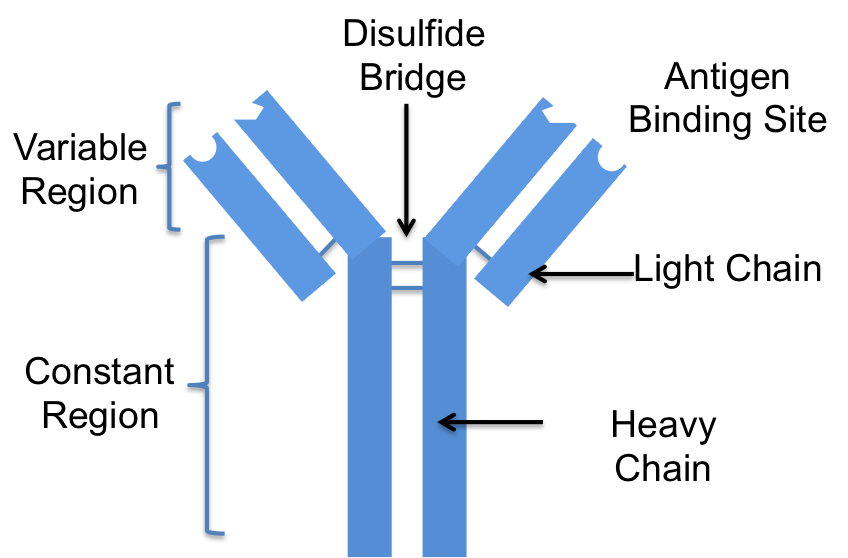
\includegraphics[width=0.7\textwidth]{antibody.png}
%     \caption[Antibody with basic structural features labeled]{Antibody with basic structural features labeled \cite{UsingAntibodiesVaccinea}}
%     \label{fig:antibody}
% \end{figure}

Many biosensors require that a "label" is attached to the biomolecule of interest and then the concentration of this label is detected and extrapolated to the concentration of the biomolecule \cite{danielsLabelFreeImpedanceBiosensors2007}. Label-free biosensors, on the other hand, directly detect the target biomolecule by measuring the changes in electrical properties of the surface of the biosensor when binding occurs. Since labelling can dramatically alter the binding properties of biomolecules and adds complexity and cost to the assay process, label-free detection is highly desirable \cite{danielsLabelFreeImpedanceBiosensors2007}, especially in point-of-care environments. The IDE's used for testing in this project use antibodies as the label-free bio-recognition element.

The concentration of the analyte in the sample can be estimated based on the number of bio-recognition events, however in order to convert the bio-recognition events into a measurable signal, a transducer mechanism is needed\cite{bhallaIntroductionBiosensors2016}. 

\subsection{Transducer Mechanisms}
There are various types of transducer mechanisms that can be used in biosensors, including optical, piezoelectric and electrochemical transducers. This project will focus on biosensors where binding events change the electrical properties of the biosensor, specifically the complex impedance. Thus, electrochemical transducers are of interest. 

Electrochemical transducers can use various analysis techniques. In potentiometric analysis, the potential of an electrode is measured against a reference electrode at zero-current \cite{magarElectrochemicalImpedanceSpectroscopy2021}. Coulometry applies a constant potential (with regard to a reference electrode) onto an electrode surface to carry out exhaustive electrolysis of an analyte \cite{magarElectrochemicalImpedanceSpectroscopy2021}. Voltammetry involves subjecting the sample to a varying potential at the electrode's surface and measuring the resulting Faradaic current \cite{magarElectrochemicalImpedanceSpectroscopy2021}. Finally, there is \ac{EIS}, which measures the complex impedance of an electrochemical system as a function of frequency \cite{magarElectrochemicalImpedanceSpectroscopy2021}. \Ac{EIS} is particularly suitable for biosensor applications where biological binding events alter the electrical properties of the electrode-electrolyte interface \cite{danielsLabelFreeImpedanceBiosensors2007}. 

\section{Fundamentals of EIS}
EIS involves applying a small sinusoidal perturbation to the \ac{DUT} and measuring the response. This can be either a voltage or current signal, \rephrase{while the other is measured}. By varying the frequency of the excitation signal, different electrochemical processes that occur at distinct time constants can be characterised.

\Ac{EIS} relies on the system acting as a linear time-invariant system, but most real-world electrochemical systems are inherently nonlinear \cite{lazanasErratumElectrochemicalImpedance2025}. To approximate linear behaviour and ensure valid results, EIS uses a small AC excitation signal, typically between 1–10 mVpp\cite{EISQualityIndicators}\cite{lazanasErratumElectrochemicalImpedance2025}. At higher amplitudes, the response deviates from ideal sinusoidal form, causing harmonic distortion and invalid measurements. However, making the excitation too small reduces signal-to-noise ratio, so 10 mVpp is commonly used to balance linearity and measurement quality.  
% Praat oor voordele van EIS bo ander metodes
A key advantage of \ac{EIS} is the ability to simulate the electrochemical system using equivalent circuit models. These models represent the various resistive, capacitive, and diffusive elements that represent the behaviour of the system \cite{lazanasErratumElectrochemicalImpedance2025}. This is due to the frequency domain nature of EIS, in comparison with other techniques such as voltammetry that works in the time-domain, thus allowing the behaviour of distinct processes that dominate at certain frequencies to be characterised \cite{lazanasErratumElectrochemicalImpedance2025}. By fitting experimental impedance data to these models, parameters such as charge transfer resistance and double-layer capacitance can be extracted, which correlate with biomolecular interactions occurring on the electrode surface \cite{danielsLabelFreeImpedanceBiosensors2007}. This capability makes \ac{EIS} a powerful tool for label-free biosensing applications. 

EIS biosensors can be categorized into two main types based on their transduction mechanism: faradaic and non-faradaic sensors.

\subsection{Faradaic vs Non-Faradaic EIS Sensors}\label{subsec:lit_review_eis_sensors}
In faradaic measurements, charge transfers occur at the electrode-solution interface and redox reactions occur on the electrode surface \cite{xieReviewAdvancementsNanoscale2020a}. The basic equivalent circuit model for faradaic sensors is the Randles circuit (Figure \ref{fig:randles_fardaic}), consisting of solution resistance ($R_s$) in series with the parallel combination of double-layer capacitance ($C_{dl}$) and charge transfer resistance ($R_{CT}$) plus Warburg impedance ($Z_w$) representing diffusion processes \cite{xieReviewAdvancementsNanoscale2020a}.

Non-faradaic measurements operate without charge-transfer reactions, functioning as capacitive sensors that detect changes in the electrical double layer capacitance. Due to the lack of charge-transfer, $R_{CT}$ becomes infinitely large, thus creating an open circuit \cite{xieReviewAdvancementsNanoscale2020a}. On solid electrodes, the observed impedance response of $C_{DL}$ differs from an ideal capacitor, thus a \ac{CPE} is used instead of $C_{DL}$ in the Randles non-fardaic equivalent circuit (Figure \ref{fig:randles_non_faradaic}).  

\begin{figure}[ht]
    \centering
    \begin{subfigure}{0.45\textwidth}
        \centering
        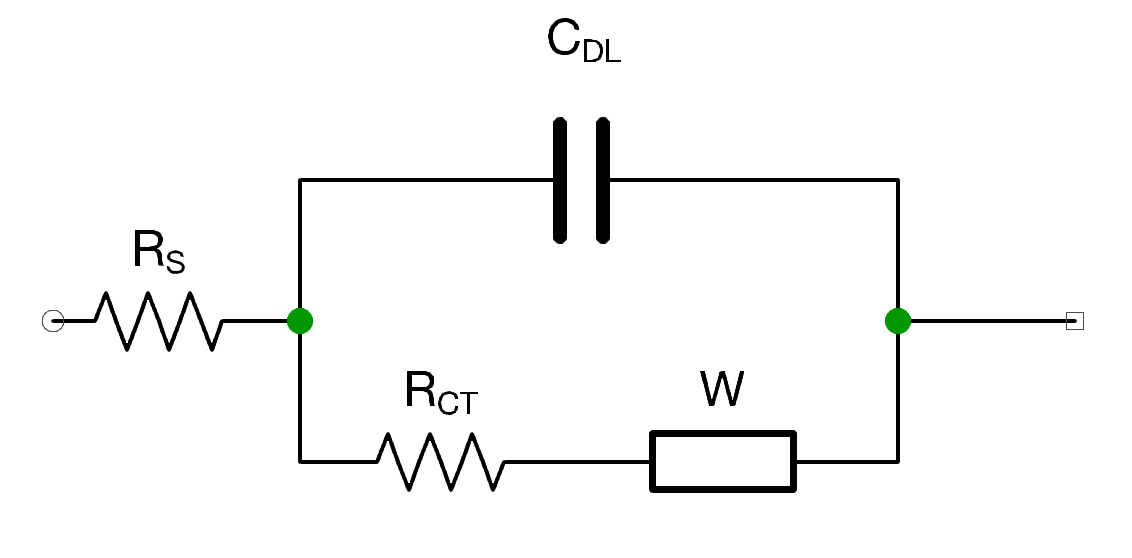
\includegraphics[width=\textwidth]{RandlesFaradaic.png}
        \caption{Faradaic Randles Circuit}
        \label{fig:randles_fardaic}
    \end{subfigure}
    \hfill
    \begin{subfigure}{0.45\textwidth}
        \centering
        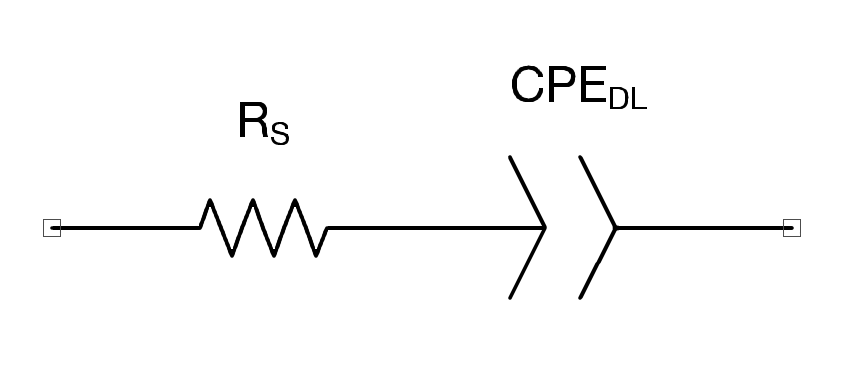
\includegraphics[width=\textwidth]{RandlesNonFaradaic.png}
        \caption{Non-Faradaic Randles Circuit}
        \label{fig:randles_non_faradaic}    
    \end{subfigure}
    \caption{Equivalent Circuits for Faradaic and Non-Faradaic EIS Biosensors}
    \label{fig:randles_circuits}
\end{figure}

\Ac{EIS} produces complex impedance data which contain both magnitude and phase information across a range of frequencies. \rephrase{This data is what allows for the characterisation of the electrochemical system and the extraction of parameters through equivalent circuit modelling.}

\section{Complex Impedance}
The complex impedance can be calculated as:
\begin{equation}
    Z(\omega) = \frac{V(\omega)}{I(\omega)} = Z'(\omega) + jZ''(\omega)
\end{equation}
where $Z'(\omega)$ is the real component representing resistive behaviour and $Z''(\omega)$ is the imaginary component representing capacitive or inductive behaviour (with $V(\omega)$ and $I(\omega)$ representing the phasor voltage and current respectively) \cite{lazanasErratumElectrochemicalImpedance2025}.

Two major ways of visualizing this complex impedance are the Nyquist and Bode representations, each highlighting different aspects of the electrochemical response.

\subsection{Nyquist Plot}
A Nyquist plot displays the negative imaginary part of impedance($Z''(\omega)$) versus the real part ($Z'(\omega)$) \cite{BodeNyquistPlot}. Each point on the plot corresponds to a particular frequency, though the frequency is not explicitly shown along the axes. For biosensing, high-frequency data points are located near the origin (low impedance), while low-frequency points are farther along the curve (high impedance). The Nyquist plot has the distinct advantage that some circuit parameters can be read directly form the plot \cite{BodeNyquistPlot}. 

A purely resistive impedance is represented as a point on the x-axis, as it has no imaginary component and is not frequency dependent. A purely capacitive impedance on the other hand is represented as a straight vertical line on the y-axis, as it has no real component and its imaginary component varies inversely with frequency \cite{BodeNyquistPlot}. The series combination of resistive and capacitive elements, thus result in a vertical line, offset from the y-axis. The parallel combination of resistive and capacitive elements, however result in a semicircular arc, as current flows though the path of least resistance \cite{BodeNyquistPlot}. At low frequencies, the capacitor acts as an open circuit resulting in the x-axis intercept (or diameter of the semi-circle) representing the magnitude of the resistive elements in the circuit. The series combination of a resistor and parallel resistor-capacitor thus results in a semicircular arc offset from the y-axis.

For simple electrochemical systems such as a Randles cell, the Nyquist plot appears as a semicircle (frequencies where charge transfer phenomena dominate) ending in a straight line tail (frequencies where mass transfer phenomena dominate) (Figure \ref{fig:randles_nyquist}) \cite{lazanasErratumElectrochemicalImpedance2025}. The series resistance ($R_s$) can be read directly from the x-axis intercept at high frequencies (closer to the origin), while the charge transfer resistance ($R_{CT}$) is given by the diameter of the semicircle in middle frequencies. At low frequencies, the Warburg impedance ($Z_w$) manifests as a 45-degree line due to diffusion-limited processes \cite{lazanasErratumElectrochemicalImpedance2025}, explaining the observed tail.

The non-faradaic Randles equivalent, however does not exhibit a semi-circle, due to the exclusion of the charge transfer resistance ($R_{CT}$) and Warburg impedance ($Z_w$). Instead, the Nyquist plot appears as a straight line with an x-axis intercept representing $R_S$. For solid electrodes, however the line is not vertical as would be expected from the series combination of a resistive and purely capacitive element \cite{xieReviewAdvancementsNanoscale2020a} (Figure \ref{fig:RandlesNonFaradaicNyquist}). The $C_{DL}$ is thus replaced with a \ac{CPE} in the circuit model to account for this non-ideal capacitive behaviour.

\begin{figure}[H]
    \centering
    \begin{subfigure}{0.45\textwidth}
        \centering
        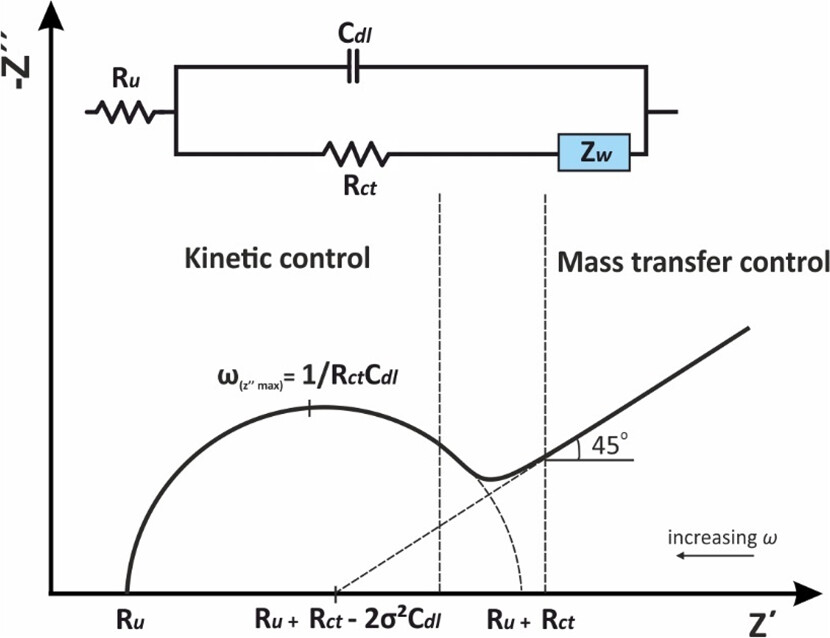
\includegraphics[width=\textwidth]{RandlesNyquist.jpeg}
        \caption[Faradaic Randles Circuit]{Faradaic Randles Circuit \cite{lazanasErratumElectrochemicalImpedance2025}}
        \label{fig:randles_nyquist_faradaic}
    \end{subfigure}
    \hfill
    \begin{subfigure}{0.45\textwidth}
        \centering
        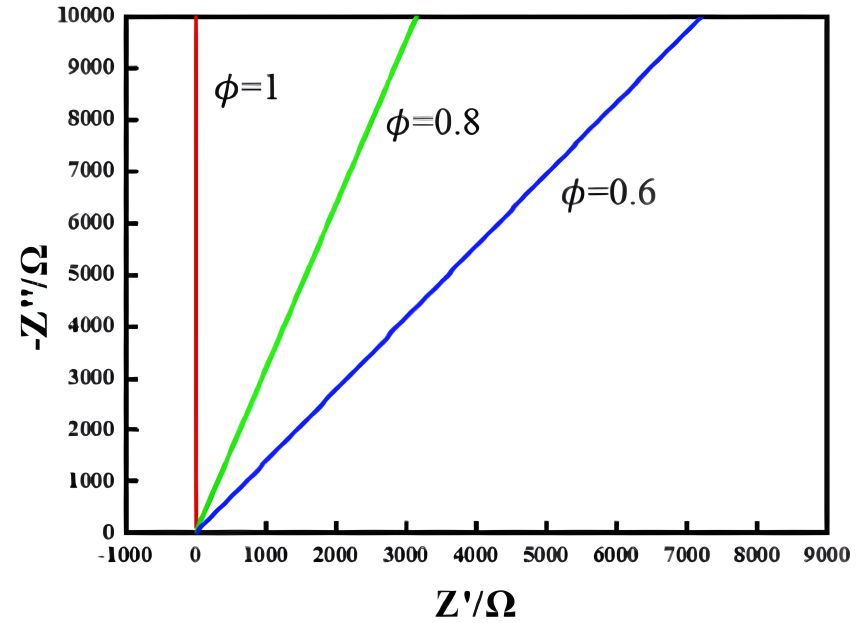
\includegraphics[width=\textwidth]{RandlesNonFaradaicNyquist.png}
        \caption[Non-Faradaic Randles Circuit]{Non-Faradaic Randles Circuit \cite{xieReviewAdvancementsNanoscale2020a}}
        \label{fig:RandlesNonFaradaicNyquist}    
    \end{subfigure}
    \caption{Nyquist Plots of Faradaic and Non-Faradaic Randles Circuits}
    \label{fig:randles_nyquist}
\end{figure}

\begin{equation}
    Z_{CPE} = \frac{1}{T(j\omega)^{\alpha}}
    \label{eq:cpe_impedance}
\end{equation}

The impedance of the \ac{CPE} is given by Equation \ref{eq:cpe_impedance}, with $\omega$ representing the angular frequency, $T$ being a constant related to capacitance, and $\alpha$ being an exponent between 0 and 1 that characterizes the deviation from ideal capacitive behaviour \cite{xieReviewAdvancementsNanoscale2020a}. $\alpha$ corresponds to the angle of the line in the Nyquist plot. When $\alpha = 1$, the \ac{CPE} behaves as an ideal capacitor, while values less than 1 indicate increasing non-ideality due to factors such as surface roughness or inhomogeneities \cite{xieReviewAdvancementsNanoscale2020a}.

An alternative representation of complex impedance data is the Bode plot.

\subsection{Bode Plots}

A Bode plot presents the magnitude, $|Z|$, and phase, $\phi$, of the impedance as functions of frequency on a logarithmic scale. The Bode magnitude plot reveals how impedance changes with frequency, while the phase plot shows the transition between capacitive ($\phi = -90^\circ$)  and resistive ($\phi = 0^\circ$) behaviour. While Nyquist plots offer direct visualization of resistive and capacitive interactions, Bode plots highlight the frequency dependence and allow clearer distinction of time constants \cite{BodeNyquistPlot}. In EIS analysis, both representations are complementary: Nyquist plots assist model-based fitting, whereas Bode plots verify consistency and highlight transition frequencies.

To obtain impedance measurements, specialised instrumentation known as impedance analysers are employed.

\section{Impedance Analysers}
Impedance analysers integrate signal generation, voltage and current measurement, and data processing to determine the complex impedance of a \ac{DUT}. In biosensing, these devices perform \ac{EIS} by applying a known AC excitation and measuring the resulting voltage and current responses over a range of frequencies. The ratio of these phasor quantities provides the frequency-dependent impedance, revealing biochemical interactions at the electrode–electrolyte interface \cite{lazanasErratumElectrochemicalImpedance2025}.

Commercial solutions such as the PalmSens4, Gamry Reference 600+, and Metrohm Autolab PGSTAT offer exceptional accuracy, broad frequency ranges (typically 10 $\mu$Hz to 1 MHz or higher), and advanced analytics including integrated equivalent circuit fitting \cite{PalmSens4}. However, these instruments are prohibitively expensive ($\approx$ \texteuro 4200 for the PalmSens4) and require significant technical expertise to interpret results. This makes them unsuitable for low-resource \ac{POC} settings where portability, cost, and ease of use are crucial \cite{pariharPointofcareBiosensorsInfectious}. Miniaturised, low-cost impedance analysers are therefore being actively developed for POC applications \cite{buscagliaSimpleZLowCostPortable2023, al-aliDesignPortableLowCost2017, ibrahimCMOSTransimpedanceAmplifier, pariharPointofcareBiosensorsInfectious}. Such designs prioritise simplicity, automation, and affordability, while maintaining sufficient frequency range and measurement accuracy to detect biological binding events.

The analogue frontend of an impedance analyser typically consists of three main subsystems: signal generation, voltage measurement, and current measurement.
\subsection{Signal Generation}\label{subsec:lit_review_excitation}
\Ac{EIS} requires the generation of a small AC excitation signal, either voltage or current, to probe the \ac{DUT} \cite{orazemTutorialElectrochemicalImpedance2020}. Generating a small current signal is difficult to do accurately and requires circuits such as the improved Howlard current pump \cite{ImprovedHowlandCurrent2020}. On the other hand, generating voltage signals are simple, and thus the method commonly used in \ac{EIS} systems \cite{orazemTutorialElectrochemicalImpedance2020}.

Voltage-based signal generation can use dedicated chips like the AD5933 or custom solutions using microcontroller-based \acp{DAC}. The AD5933 offers integrated frequency sweeps and impedance measurement, making it attractive for simple implementations \cite{AD5934TestUpdate}. However, it has several critical drawbacks. The chip has a DC offset between excitation and measurement stages, which is problematic because biosensing requires bipolar signals with no DC component \cite{seoaneAnalogFrontendEnables2008}. DC bias causes charge accumulation at the electrode–electrolyte interface, establishing a net electrochemical potential that drives unwanted redox reactions. Over time, these parasitic reactions alter the interfacial chemistry and change the electrode's impedance characteristics, obscuring the properties that non-faradaic \ac{EIS} aims to measure. The AD5933 also lacks direct voltage measurement capability and has a minimum measurable impedance of 1 k$\Omega$, further limiting its suitability for biosensing applications.

In contrast, a \ac{DAC} and \ac{ADC} solution implemented on a microcontroller allows precise control of excitation signals, flexible signal processing, and easier integration with multiplexing subsystems. 

When generating sinusoidal signals using a \ac{DAC}, the output is not a smooth analogue waveform but rather a series of discrete voltage steps. These steps introduce high-frequency components and harmonics not present in the original signal. Without filtering, they may interfere with downstream circuitry or cause aliasing during analog-to-digital conversion. An anti-aliasing filter (AA filter), typically a \ac{LPF}, is placed after the \ac{DAC} output to remove high-frequency content and smooth the signal.

The dynamic range of a \ac{DAC}, expressed in decibels, determines the smallest signal it can produce above its noise floor and is given by:
\begin{equation}
    \text{Dynamic Range} = 6.02n + 1.76 
    \label{eq:dac_range_lit}
\end{equation}
where $n$ is the number of bits of resolution \cite{gaddyDYNAMICPERFORMANCETESTING}. The AA filter must attenuate high-frequency components sufficiently so that aliased content falls below this noise floor, whilst maintaining a flat passband response to avoid distorting the intended output's amplitude or phase.

For systems generating signals across wide frequency ranges, a fixed-frequency AA filter becomes unsuitable. A single cutoff frequency cannot accommodate both low and high signal frequencies without either excessive attenuation or inadequate filtering. Variable AA filters address this by allowing dynamic cutoff adjustment. Many require changing resistor values to set the cutoff frequency, which is impractical for rapid frequency changes. Clock-tunable filters, which adjust their cutoff based on an external clock signal, thus offer a more flexible solution for wide frequency sweeps.

While some impedance analyser designs infer the applied voltage by using the known characteristics of the excitation stage \cite{buscagliaSimpleZLowCostPortable2023}, this fails to account for parasitic resistances, stray capacitance, drift, and environmental changes. Direct measurement captures all these variations, leading to reliable impedance calculations. This is vital in low-voltage biosensing where small changes significantly affect calculated impedance.

\subsection{Voltage Measurement}\label{subsec:lit_review_v_meas}
Two common circuits for differential voltage measurements are differential op-amps and instrumentation amplifiers. Differential op-amps are simple and cost-effective but are susceptible to common-mode noise and offset errors \cite{technologyWhatAreDrawbacks2024}. They also have relatively low input impedance, which loads the signal source and affects measurements \cite{technologyWhatAreDrawbacks2024}. Instrumentation amplifiers are specifically designed for high-precision differential measurement. They provide superior common-mode rejection, high input impedance, and excellent accuracy even with small signals in noisy environments \cite{InstrumentationAmplifierOperational}. This is due to their three op-amp design, making them particularly suitable for biosensing where signals can be very small and minimising interference is critical.

Amplifying the measured voltage to fully utilise the \ac{ADC}'s linear range enhances both sensitivity and resolution. By maximising the voltage swing within the \ac{ADC}'s input range, the system can discriminate smaller changes in sensor response, allowing for better detection of low-concentration analytes. However, amplification introduces trade-offs related to gain-bandwidth product, which limits usable bandwidth at higher gains. Multi-stage amplification distributes gain across several stages, allowing higher overall gain whilst maintaining adequate bandwidth across the measurement frequency range.

While the measured voltage is relatively constant, the current through the \ac{DUT} can vary dramatically depending on its impedance. Thus, accurate current measurement is essential for determining the impedance of the \ac{DUT}.

\subsection{Current Measurement}
Two primary approaches to measuring current exist, namely shunt resistor based measurement and transimpedance amplifier based measurement.

The most basic method places a small known precision resistor (shunt resistor) in series with the current path and measures the voltage drop across it. Ohm's Law then gives the current. This approach is cheap and easy to implement but has severe drawbacks. The voltage drop across the resistor directly reduces the magnitude of the applied perturbation to the \ac{DUT}, impacting measurements. For biosensing, where signal levels are already low, even small drops significantly affect sensitivity.

A \ac{TIA} on the other hand, converts input current to a proportional output voltage without introducing significant voltage drop across the \ac{DUT}. The \ac{TIA} makes use of the following properties of op-amps:
\begin{equation}
    V_n \approx V_p
    \label{eq:opamp_V}
\end{equation}
\begin{equation}
    I_n \approx I_p \approx 0
    \label{eq:opamp_I}
\end{equation}
where $V_n$ and $V_p$ are the voltages at the inverting and non-inverting inputs respectively, and $I_n$ and $I_p$ are the input bias currents. The positive input (connected to the \ac{DUT}) is driven to the same potential as the negative input (ground or reference voltage), thereby ensuring a low-impedance path for the current. Conversely, Equation \ref{eq:opamp_I} ensures that the TIA has a high input-impedance and that the current from the sensor flows entirely through the feedback resistor. The output voltage is then given by:
\begin{equation}
    V_{out}=I_{in} \times R_{feedback}
    \label{eq:tia_gain}
\end{equation}
The \ac{TIA} has the advantage that unlike a shunt resistor, the feedback resistor can be large without affecting the applied signal.

In biosensing with fixed voltage perturbation, current varies dramatically depending on the \ac{DUT}'s impedance; from nanoamperes at high impedance to milliamperes at low impedance. A fixed-gain amplifier is impractical across this dynamic range. It would either saturate at high currents or provide insufficient resolution at low currents. Variable gain amplification, achieved through switchable feedback resistors in the \ac{TIA} or \acp{PGA} in subsequent stages, allows the system to adapt to current magnitude. This ensures output voltage remains within the optimal range for the \ac{ADC} whilst maximising measurement resolution.

\todo{Add linking sentence}

\section{Related Works}

\label{chap:literature_review}
\graphicspath{{design/fig/}}

\chapter{Design}

\section{Functional Design Overview}
Discuss wat ons wil bereik en hoe ons dit gan opbreek. Beskryf hoe die circuit die beginsels van biosensors en EIS in ag moet neem, basies wat dit moet doen, hoekom multiplexing en ja dan hoe daai overall doel in gedeeltes opgebreek word.

\subsection{DUT}

\subsection{Multiplexer}

\subsection{Excitation}

\subsection{Voltage Measurement}

\subsection{Current Measurement}

\subsection{DSP (STM)}

\subsection{User Interface (ESP etc)}

\section{Detailed Design}
Gaan meer in diepte oor circuitry maar steeds met generic/ideal coponents. Cover circuitry van elke section, design requirements etc soos 10mV excitation bv. Wat wil ons bereik en dan hoe daai translate na technical requirements en dan die circuitry. Wys LT Spice circuits en sims van elke seksie en combined. Cost is n spec (<R4500).

\subsection{DUT}
Data van Dr Ebrahim, en dan kry circuit model van daai af.

\subsection{Voltage Reference}
Verduidelik dat ons bipolar signaling kort sonder DC offset, en ipv +- 1.65V doen ons 1.65V virtual ground.

\subsection{Excitation Stage}
Verduidelik hoekom ons 3.3V output signal van DAC gebruik (maximise range theory). Verduidelik hoekom ons 10mV soek gebasseer op DUT circuit model. Gee brief overview van beginsels van opamp em somme. Verduidelik dan hoekom LPF Anti Aliasing nodig is gebasseer op Frequency domain theory en al daai. Calcs rondom hoe naby aan signal freq cutoff moet wees, dus variable LPF. Te expenny om self te bou dus eerder IC. Was voor en na Filter van DAC sims.

\subsection{Voltage Measurement}
Why is voltage measurement needed when we already know our output voltage. Discuss what to consider when amplifying signal. Discuss LPF en hoekom n volle variable een nie needed is nie (dit is meestal vir noise nie vir anti aliasing van sampling nie, want DAC AA behoort dit te keer).

\subsection{Current Measurement}
Beskryf hoekom current measurement so belangrik is. Wat ons range van currents is. Beskryf beginsels van TIA including somme en circuit analysis. Dan hoekom TIA nie al die amplifications doen nie en why PGA needed is. Raak dan briefly ook op die LPF beginsel selfde as voltage.

\subsection{Multiplexing}
Discuss why multiplexing needed (both why multiple sensors are useful and why not just dedicated circuitry for each sensor, including why thats not needed). Discuss options that I considered and why we settled on signal relays. Briefly discuss tree design and why that saves on relays (Double pole double throw vs net manually connect disconnect each relay to central line).

\subsection{DSP}
Discuss why DSP needed, why microcontroller and not other DSP. Beskryf basies hoe ons filtering gaan doen etc. Die formules en konsepte van freq domain en hoe ons capacitance calc en dan na concentration gaan. Los die details van code en libraries en issues vir Firmware Design section.

\subsection{User Interface}
Baie briefly discuss wat ons vereis van

\section{Component Selection}
Watse komponente ons kies, why en watse aspekte ons consider het en hoekom daai specs belangrik is. How een komponent die ander beinvloed. Wys sims met spesifieke komponent seleksies. Wys calcs vir passive compoinent selections.

\section{PCB Design}
Beskryf filosofie en idees wat mee ingegaa het. Briefly discuss general PCB design principles wat design geguide het (Analogue ground plane etc). Beskryf beperkings van PCB manufactures wat inag geneem moes word (PCB size, layers, trace width via diamtre etc.). Noem briefly hoekom PCB in China eerder as Uni laat maak. Gaan deur design logic en discuss probleem met TIA. Include maybe final PCB diagram en langs dit foto van manufactured PCB.

\section{Firmware Design}
Inculde flow diagram.

\subsection{ESP}
Vertel van wat ons wil bereik en hoekom. Discuss libraries used. Discuss maybe issues rondom C6 en hoe dit gesolve is en hoekom die C6 steeds die rgete keuse was.

\subsection{STM}
Probleme met arm library te groot. Discuss met flow chart hoe DMA en als met DAC en ADC interact en dan UART en badies program flow. Delve into limits van STM en maybe briefly setup van DAC en ADC.

\label{chap:design}
\graphicspath{{testing_and_validation/fig/}}

\chapter{Testing \& Validation}

The testing and validation process was structured to systematically verify the functionality of the impedance analyser, progressing from subsystem verification to complete system integration and finally calibration and validation with actual biosensors. This methodical approach allowed for the identification and correction of issues at each stage, ensuring that problems could be isolated and resolved before integration with more complex subsystems.

% Testing began with fundamental verification of the assembled PCB, followed by individual subsystem characterisation. Once subsystem functionality was established, the complete analogue frontend was tested as an integrated system. Finally, the device was calibrated against the PalmSens4 impedance analyser and validated using biosensors with buffer solutions.

\section{PCB Testing}

Upon receiving the assembled PCB visual inspection and continuity testing confirmed no obvious short circuits or discontinuities. The ESP32's onboard battery charging circuit was confirmed to supply a stable 3.3 V rail to all digital and analogue components. The virtual ground reference circuit was measured at exactly 1.650 V. The TPS61072 boost converter successfully provided a stable 5 V supply for the LTC1069 anti-aliasing filter.

Next, each subsystem was tested individually whilst other subsystems remained disconnected. This approach allowed for precise characterisation of each stage's performance and simplified fault diagnosis.

\subsection{Excitation Stage} 
The excitation stage was tested using a signal generator providing a 3 Vpp input signal and an oscilloscope to measure the attenuated output. Unfortunately, the LTC1069 anti-aliasing filter was found to be dead-on-arrival. Given the significant lead times for component procurement and project time constraints, it was not feasible to order a replacement. The filter was therefore bypassed, and the excitation stage was tested without it. Whilst this introduces higher-frequency components from the DAC's stairstepping, the synchronisation of DAC generation and ADC sampling in the final system helps to minimise the impact on measurements.

The attenuation stage was characterised across the full frequency range from 1 Hz to 100 kHz. The resulting signal was measured at ~10.33 mV, giving a 290 V/V attenuation. This is close to the designed 300 V/V with the variation likely due to component tolerances.

% Figure \ref{fig:excitation_freq_response} shows the frequency response, which exhibits a flat gain and phase across the measurement range.
% Move fig to appendix
% \begin{figure}[H]
%     \centering
%     % \includegraphics[width=0.8\textwidth]{ExcitationFreqResponse.png}
%     \caption{Excitation Stage Frequency Response}
%     \label{fig:excitation_freq_response}
% \end{figure}

\subsection{Voltage Measurement Stage} 
For the voltage measurement stage, both the INA331 instrumentation amplifier and TLV9061 gain stage were tested separately. The INA331 was tested using a 200mV input signal to minimise noise. It performed as expected, with no measurable gain roll-off at 100 kHz and a phase shift of -5\textdegree, which is close to the expected -4.6\textdegree based on simulations.

Initial testing of the TLV9061 stage showed a completely unstable system. Investigation uncovered a critical oversight in the PCB design. The TLV9061 op-amp symbol used in KiCad had a different pinout than the LTspice model used for simulation, resulting in the inverting and non-inverting inputs being swapped. This was corrected through careful trace cutting and wire jumpers, and the corrected schematic was updated in KiCad for future PCB revisions. After this modification, the TLV9061 stage performed well, exhibiting a -8.7° phase shift at 100 kHz compared to the expected -3.4°. The larger-than-expected phase shift can be attributed to several factors including the additional parasitic capacitance introduced by the rework, tolerances in the op-amp's gain-bandwidth product, and PCB layout effects not fully captured in simulation. The measured gain roll-off at 100 kHz was less than 0.2 dB. 

Overall, the voltage measurement stage's performance closely matched expectations, with the phase discrepancies remaining well within acceptable limits for accurate impedance measurements if properly calibrated for.

\todo{Insert Table wat cutoff en 100kHz summarise vir elke afdeling en dan langs dit grafiek wat responses van elke substage wyse op eenm grafiek}


\subsection{Current Measurement Stage} 
The current measurement stage required the most extensive testing due to its complexity and switchable gain configurations. Significant concerns existed regarding the TIA functionality given the extremely small 0.4 mm pitch BGA package of the OPA3S328, however testing confirmed it operated correctly.

The TIA was characterised by applying known voltages across resistors of known values, allowing the input current to be calculated. The TIA output voltage was then measured to determine the transimpedance gain across the full frequency range. Whilst the resistor values were measured using a standard multimeter (rather than a kelvin sens connection) and the resistor's parasitic inductance and capacitance was ignored, this characterisation served primarily for functional validation, as final calibration would be performed against the PalmSens4. 

At $R_f = 37.5\,\Omega$, the TIA exhibited a gain of 37.73 V/V with a phase shift of -4.4\textdegree and gain reduction of 0.74 dB at 100 kHz. At the larger feedback resistor value of $R_f = 7.5\,k\Omega$, the gain averaged at 7427. Interestingly, both phase shift and gain reduction  at 100 kHz were less pronounced at -3.5\textdegree and \textless 0.1 dB respectively. This is possibly due to slight peaking.

Stability was verified by connecting a simplified Randles equivalent circuit with a constant capacitance of \SI{1.47}{\micro F} and resistance of $12 \Omega$, approximating the expected biosensor characteristics. A 10 mVpp signal was applied to the equivalent circuit and swept from 1 Hz to 30 MHz while monitoring the TIA output for oscillations, ringing, or excessive peaking in the frequency response. No instability was observed, confirming the theoretical analysis in Section \ref{subsec:design_cur}.

The PGA113 was measured at each gain setting from 1 V/V to 200 V/V for each measurement frequency. Table \ref{tab:pga_performance} shows the measured gain and phase shift at 100 kHz for each setting. As expected, the phase shift is noticable at higher gain settings, however the higher gains will primarily be used at lower frequencies where the phase shift is negligible. These gain and phase shift values were incorporated into the calibration procedure to ensure accurate impedance calculations.

\begin{table}[H]
\centering
\caption{PGA113 Performance at 100 kHz}
\label{tab:pga_performance}
\begin{tabular}{|c|c|c|c|c|}
\hline
\textbf{Gain Setting} & \textbf{Maximum Gain} & \textbf{100kHz Gain} & \textbf{Gain Reduction} & \textbf{100kHz Phase Shift} \\
\textbf{(V/V)} & \textbf{(V/V)} & \textbf{(V/V)} & \textbf{(dB)} & \textbf{(\textdegree)} \\
\hline
1 & 1.00 & 0.92 & -0.74 & -0.8 \\
\hline
2 & 2.00 & 1.84 & -0.71 & -2.132 \\
\hline
5 & 4.98 & 4.57 & -0.74 & -1.634  \\
\hline
10 & 9.97 & 9.15 & -0.74 & -2.613 \\
\hline
20 & 21.60 & 21.52 & -0.03 & -5.619 \\
\hline
50 & 54.00 & 53.44 & -0.09 & -7.491 \\
\hline
100 & 99.92 & 92.18 & -0.70 & -14.79 \\
\hline
200 & 198.06 & 173.17 & -1.17 & -25.73 \\
\hline
\end{tabular}
\end{table}

The final TLV9061 amplification stage in the current measurement path was modified using the same trace cutting and rewiring procedure as the voltage measurement stage. Measurements confirmed no measurable difference in performance compared to the voltage measurement path, ensuring that gain reductions and phase shifts cancel out during impedance calculation as designed.

\section{System Calibration}

With all subsystems verified individually, the system was integrated and calibrated. The complete analogue frontend was tested using passive test cells, initially with a signal generator providing the excitation. Once analogue system stability and measurement accuracy were confirmed, the STM32 was used to generate DAC signals and acquire responses with the ADCs.

The STM32's ADC offsets were calibrated using the built-in functions. The gradients were determined by applying a series of known voltages using a bench power supply, with each voltage verified using an oscilloscope and multimeter. Similarly, the DAC output was measured, and the centre point of the generated signal adjusted from 2048 to 2009 to account for the constant voltage offset in the excitation stage attenuation. This ensured that the analogue output was precisely centred at 1.65 V, ensuring the biosensor is not biased with a DC voltage.

The DAC's frequency generation capability was verified by measuring the output waveform at each test frequency using an oscilloscope. Frequency was confirmed to be accurate across the entire range, validating the timer configuration and DMA-based waveform generation. 

Initial calibration attempts using precision resistors measured with the PalmSens4 across the full frequency range (to account for parasitic impedances) proved problematic. Each TIA and PGA gain combination was calibrated separately using these measurements. However, when testing Randles equivalent circuits or actual biosensors, the frequency-dependent impedance characteristics resulted in unacceptably large error margins. \rephrase{The fixed PGA gain used during calibration did not match the actual measurement conditions, where gain settings vary with frequency to maintain optimal ADC range utilisation.}

This necessitated a revised calibration approach. The gain settings for each frequency were pre-programmed to match the expected impedance range based on PalmSens4 characterisation of the biosensors. Each analogue frontend stage was then characterised across all frequencies and gain settings. The measured gain and phase data was smoothed using a MATLAB script to eliminate measurement noise, and compiled into a comprehensive calibration table which was uploaded to the ESP32. Finally, a non-faradaic Randles equivalent test cell was measured simultaneously with both the BioPal and PalmSens4, allowing the BioPal's response to be calibrated against the reference instrument. This approach accounts for the complete signal chain at actual operating conditions, significantly improving accuracy.

It was found that at low frequencies (200Hz and below), the lack of filtering in the excitation phase, lead to significant aliasing. Due to the \ac{DUT}'s lower impedance at higher frequencies, the aliased high-frequency components dominated the response, leading to clipping at high gain settings or conversely, very low signal levels at the frequency of interest for low gain settings.

\section{Biosensor Validation}

The final validation stage involved measurements on actual biosensors using phosphate buffered saline (PBS) solution and bovine serum albumin (BSA) protein. 

% PBS 1× was selected as the electrolyte solution due to its physiological ionic strength and pH (7.4), which closely mimics the conditions in bodily fluids and provides a stable, well-characterised electrochemical environment for biosensor operation.

Figure \ref{fig:pbs_concentrations} shows impedance measurements of the biosensor in different PBS concentrations, demonstrating the BioPal's ability to clearly distinguish between solution conductivities. The impedance magnitude decreases with increasing PBS concentration as expected, confirming the device's sensitivity to electrochemical changes.

\begin{figure}[H]
    \centering
    % \includegraphics[width=0.8\textwidth]{PBSConcentrations.png}
    \caption{Biosensor Impedance Response to Different PBS Concentrations}
    \label{fig:pbs_concentrations}
\end{figure}

Whilst testing with immobilised antibodies and actual protein antigens would provide the most direct validation of biosensing capability, such tests were beyond the scope of this project due to laboratory safety restrictions, cost constraints, and limited time. Instead, BSA was used as a surface-binding protein to simulate antibody-antigen interactions. BSA is a common blocking protein that readily adsorbs to gold electrode surfaces, creating a protein layer that alters the interfacial impedance characteristics. This mimics the effect of antibody-antigen binding on the electrode surface, allowing validation of the device's ability to detect surface-based electrochemical changes rather than bulk solution properties.

The measurement protocol involved establishing a baseline impedance measurement in PBS 1×, removing the PBS and adding BSA solution to the electrode well, allowing 20 minutes for protein adsorption, flushing the electrode three times with fresh PBS 1× to remove unbound protein whilst maintaining the same solution characteristics, and finally performing a second impedance measurement.

Measurements were performed at each step using both the BioPal and the PalmSens4 for direct comparison. Figure \ref{fig:bsa_comparison} shows the impedance magnitude and phase measurements from both instruments before and after BSA binding. 
% The BioPal successfully detected the impedance increase following BSA adsorption, demonstrating its capability to measure surface-based electrochemical changes relevant to biosensing applications.

% 3 seperate figures with subfigures (not minipages) showing the change in magnitude and phase for both instruments
\begin{figure}[H]
    \centering
    \begin{subfigure}{0.48\textwidth}
        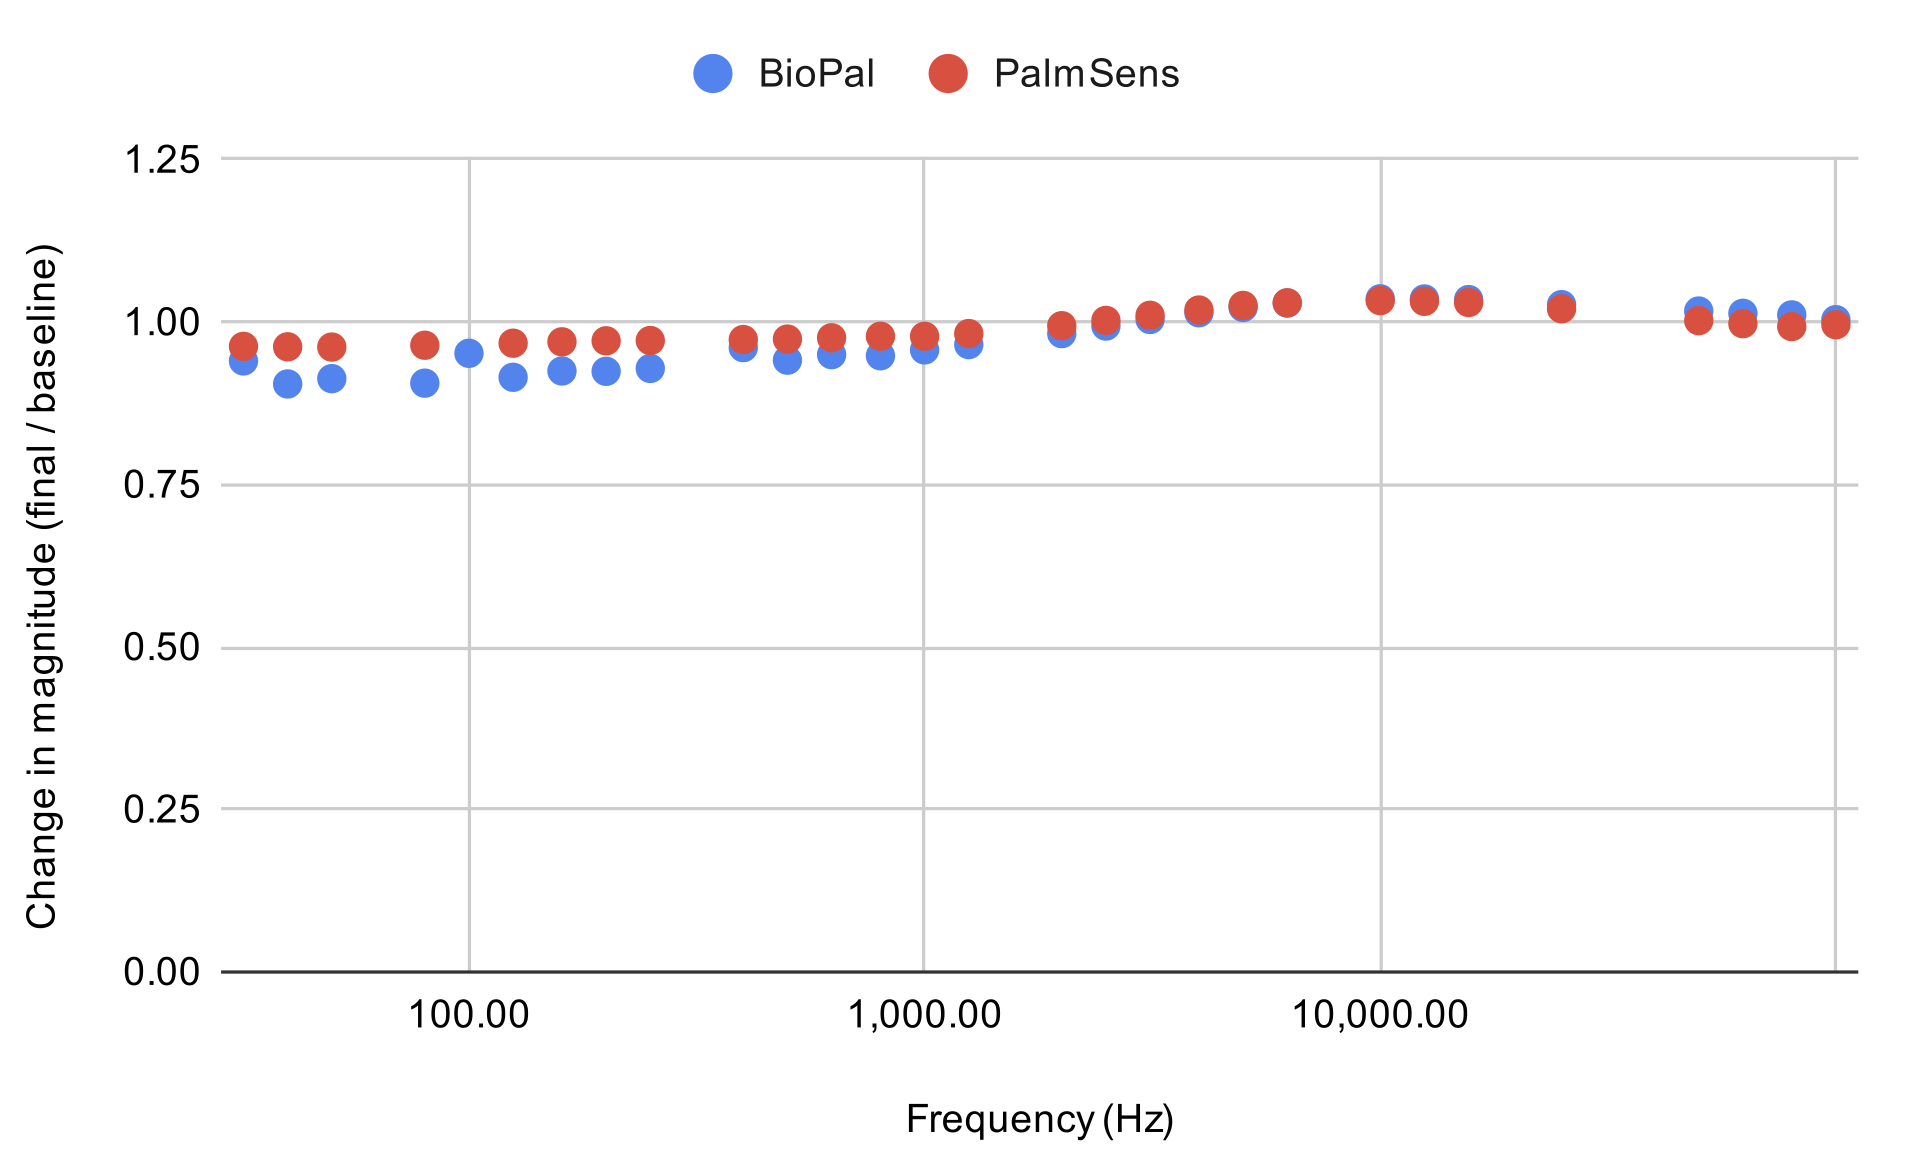
\includegraphics[width=\textwidth]{2g:100mL mag.png}
        \caption{Change in Impedance Magnitude}
        \label{fig:2g_mag}
    \end{subfigure}
    \hfill
    \begin{subfigure}{0.48\textwidth}
        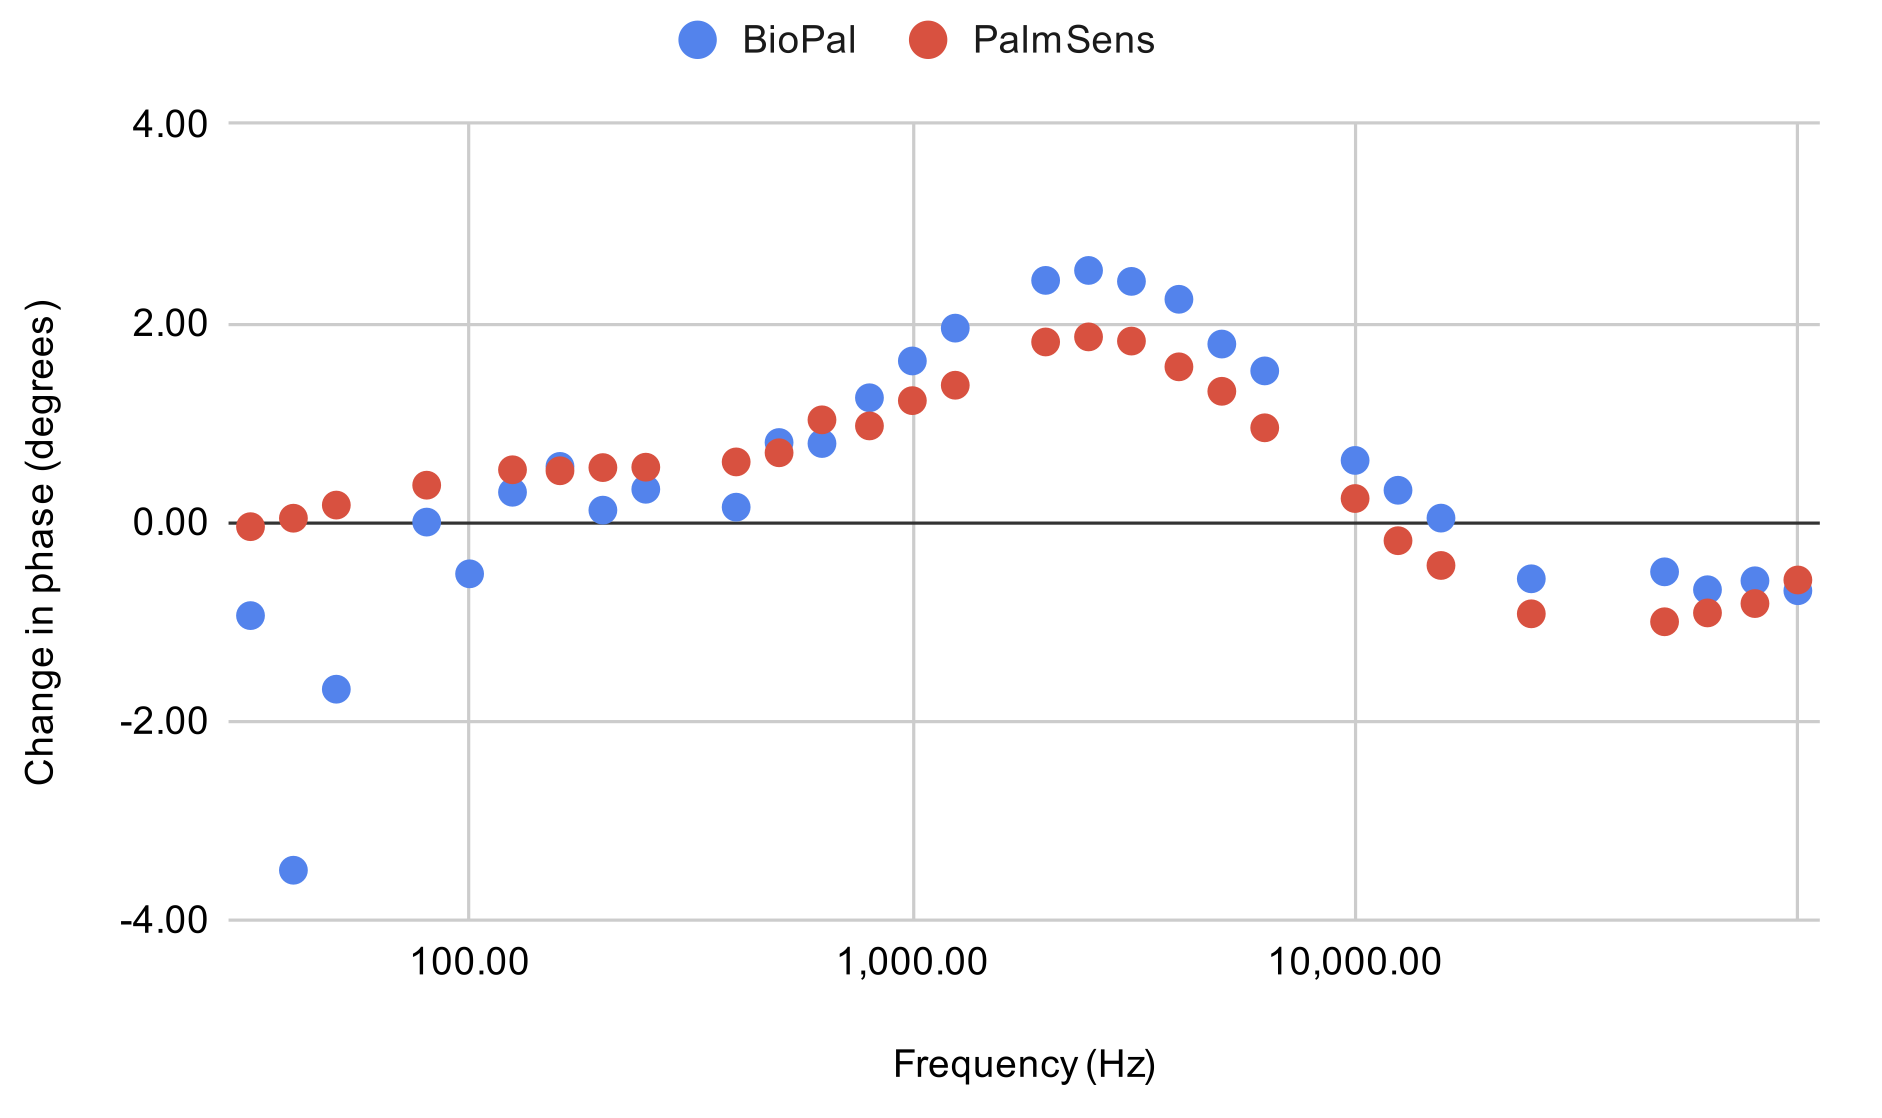
\includegraphics[width=\textwidth]{2g:100mL phase.png}
        \caption{Change in Impedance Phase}
        \label{fig:2g_phase}
    \end{subfigure}
    \caption{IDE Impedance Response to 2g/100mL BSA Binding Measured by BioPal and PalmSens4}
    \label{fig:2g_bsa_comparison}
\end{figure}

% 5g/100mL BSA
\begin{figure}[H]
    \centering
    \begin{subfigure}{0.48\textwidth}   
        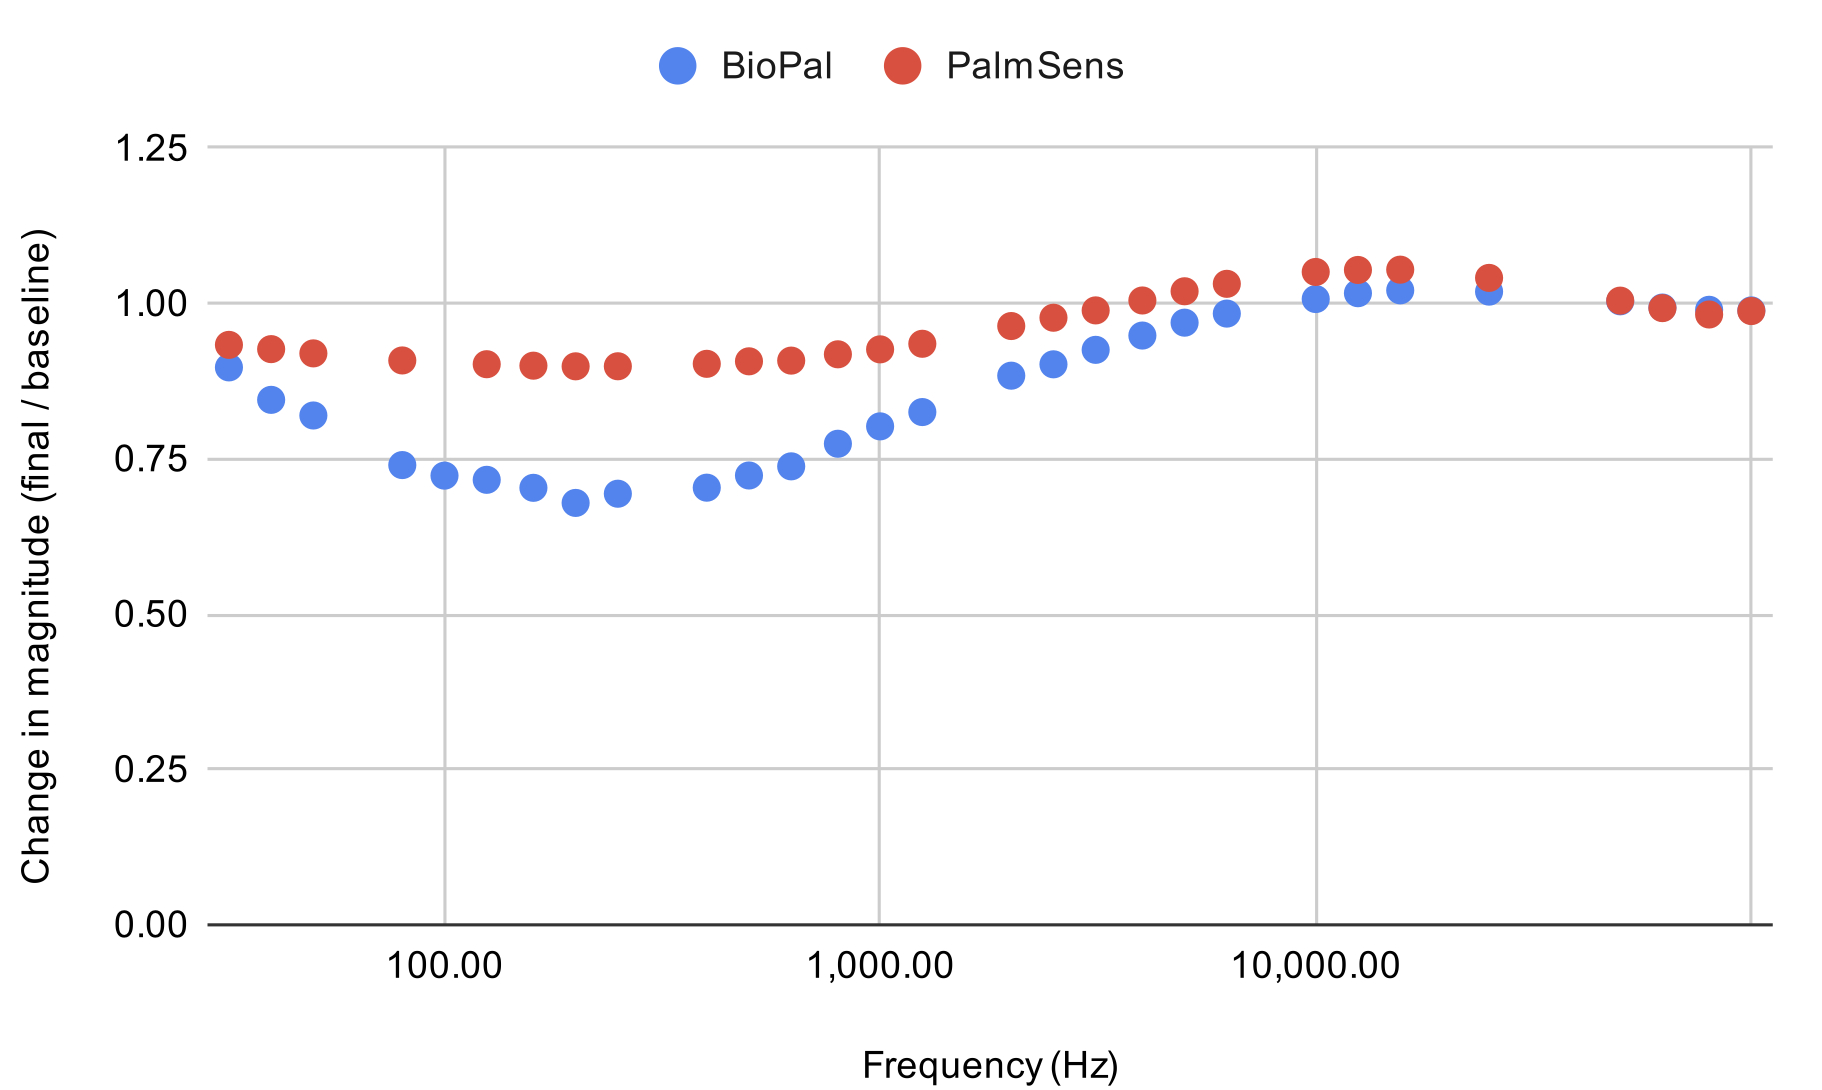
\includegraphics[width=\textwidth]{5g:100mL mag.png}
        \caption{Change in Impedance Magnitude}
        \label{fig:5g_mag}
    \end{subfigure}
    \hfill
    \begin{subfigure}{0.48\textwidth}
        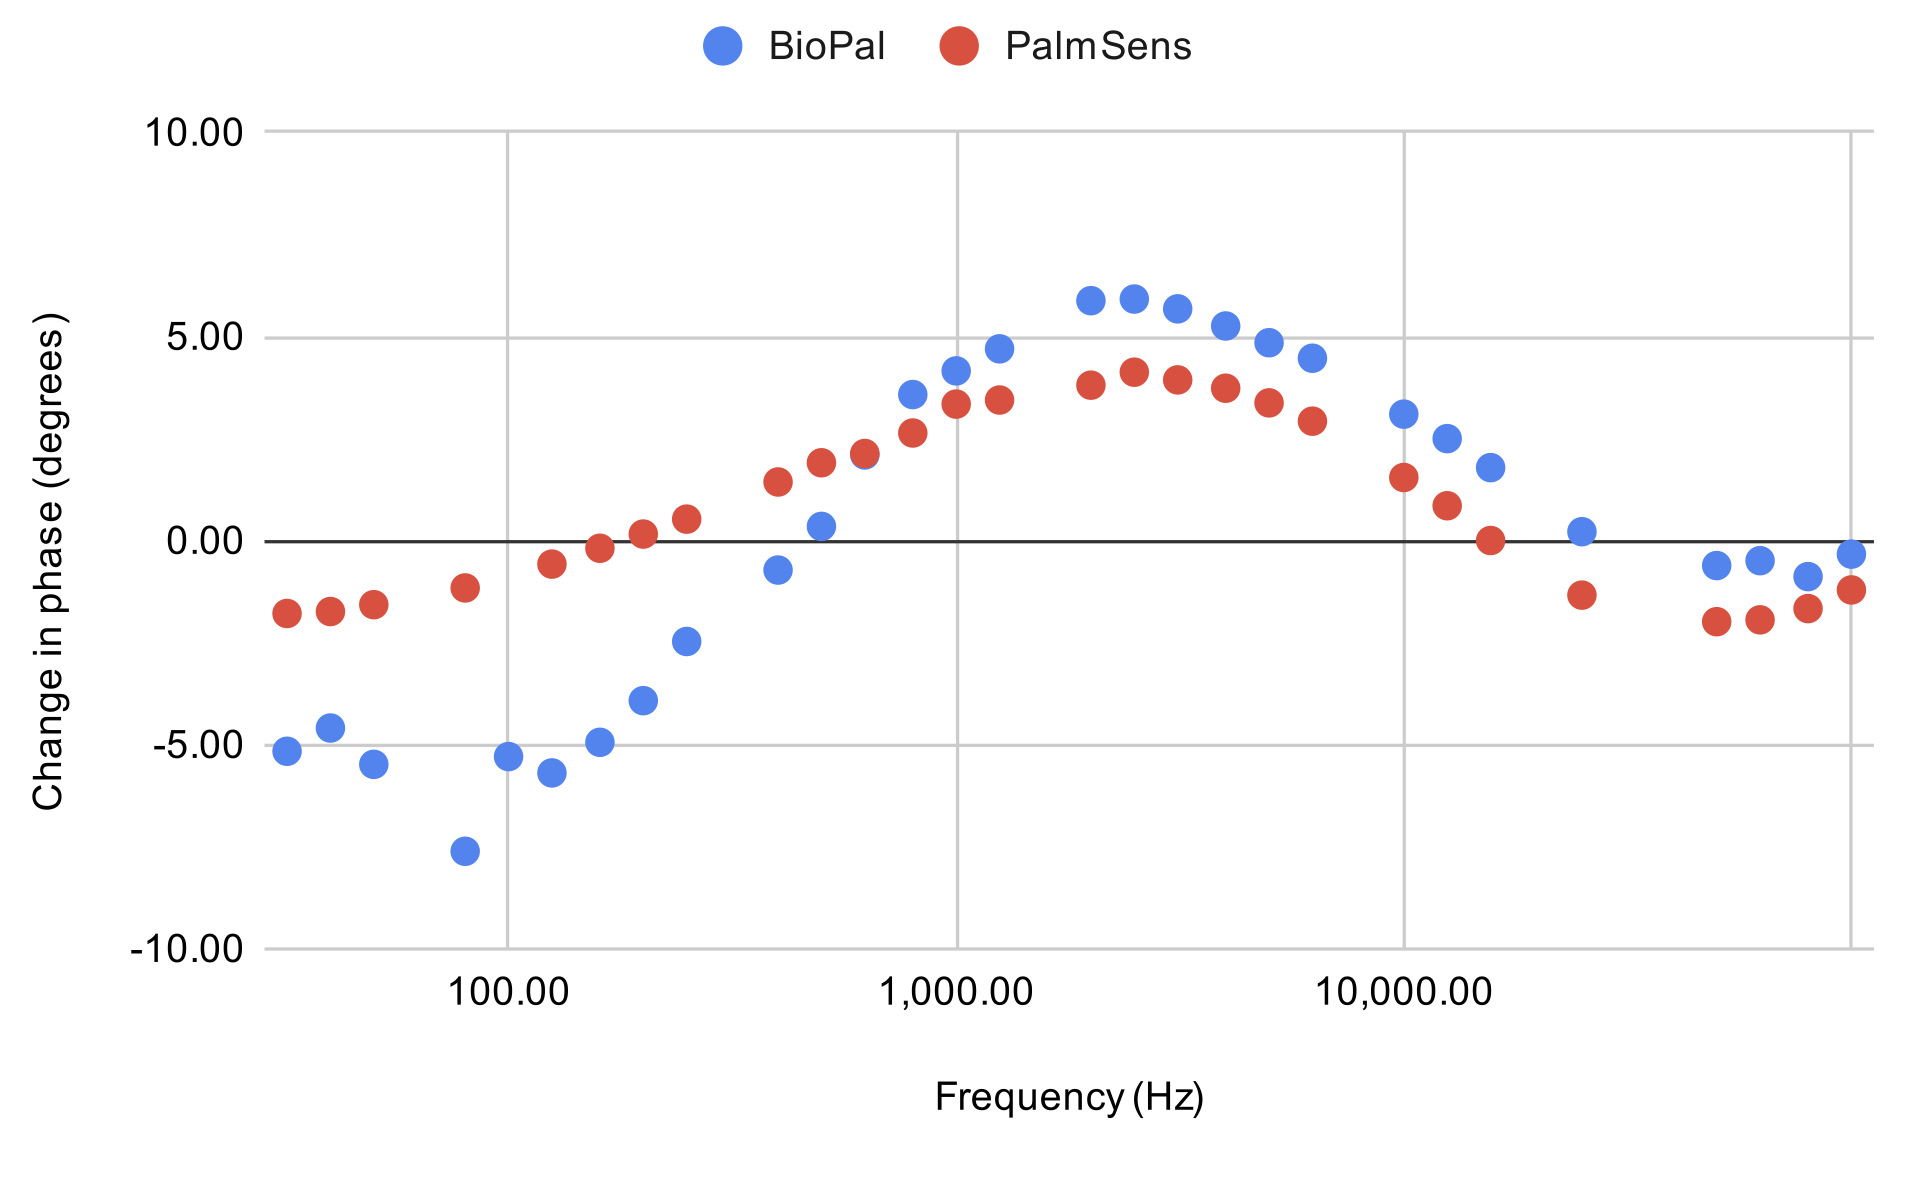
\includegraphics[width=\textwidth]{5g:100mL phase.png}
        \caption{Change in Impedance Phase}
        \label{fig:5g_phase}
    \end{subfigure}
    \caption{IDE Impedance Response to 5g/100mL BSA Binding Measured by BioPal and PalmSens4}
    \label{fig:5g_bsa_comparison}
\end{figure}

% 10g/100mL BSA
\begin{figure}[H]
    \centering
    \begin{subfigure}{0.48\textwidth}
        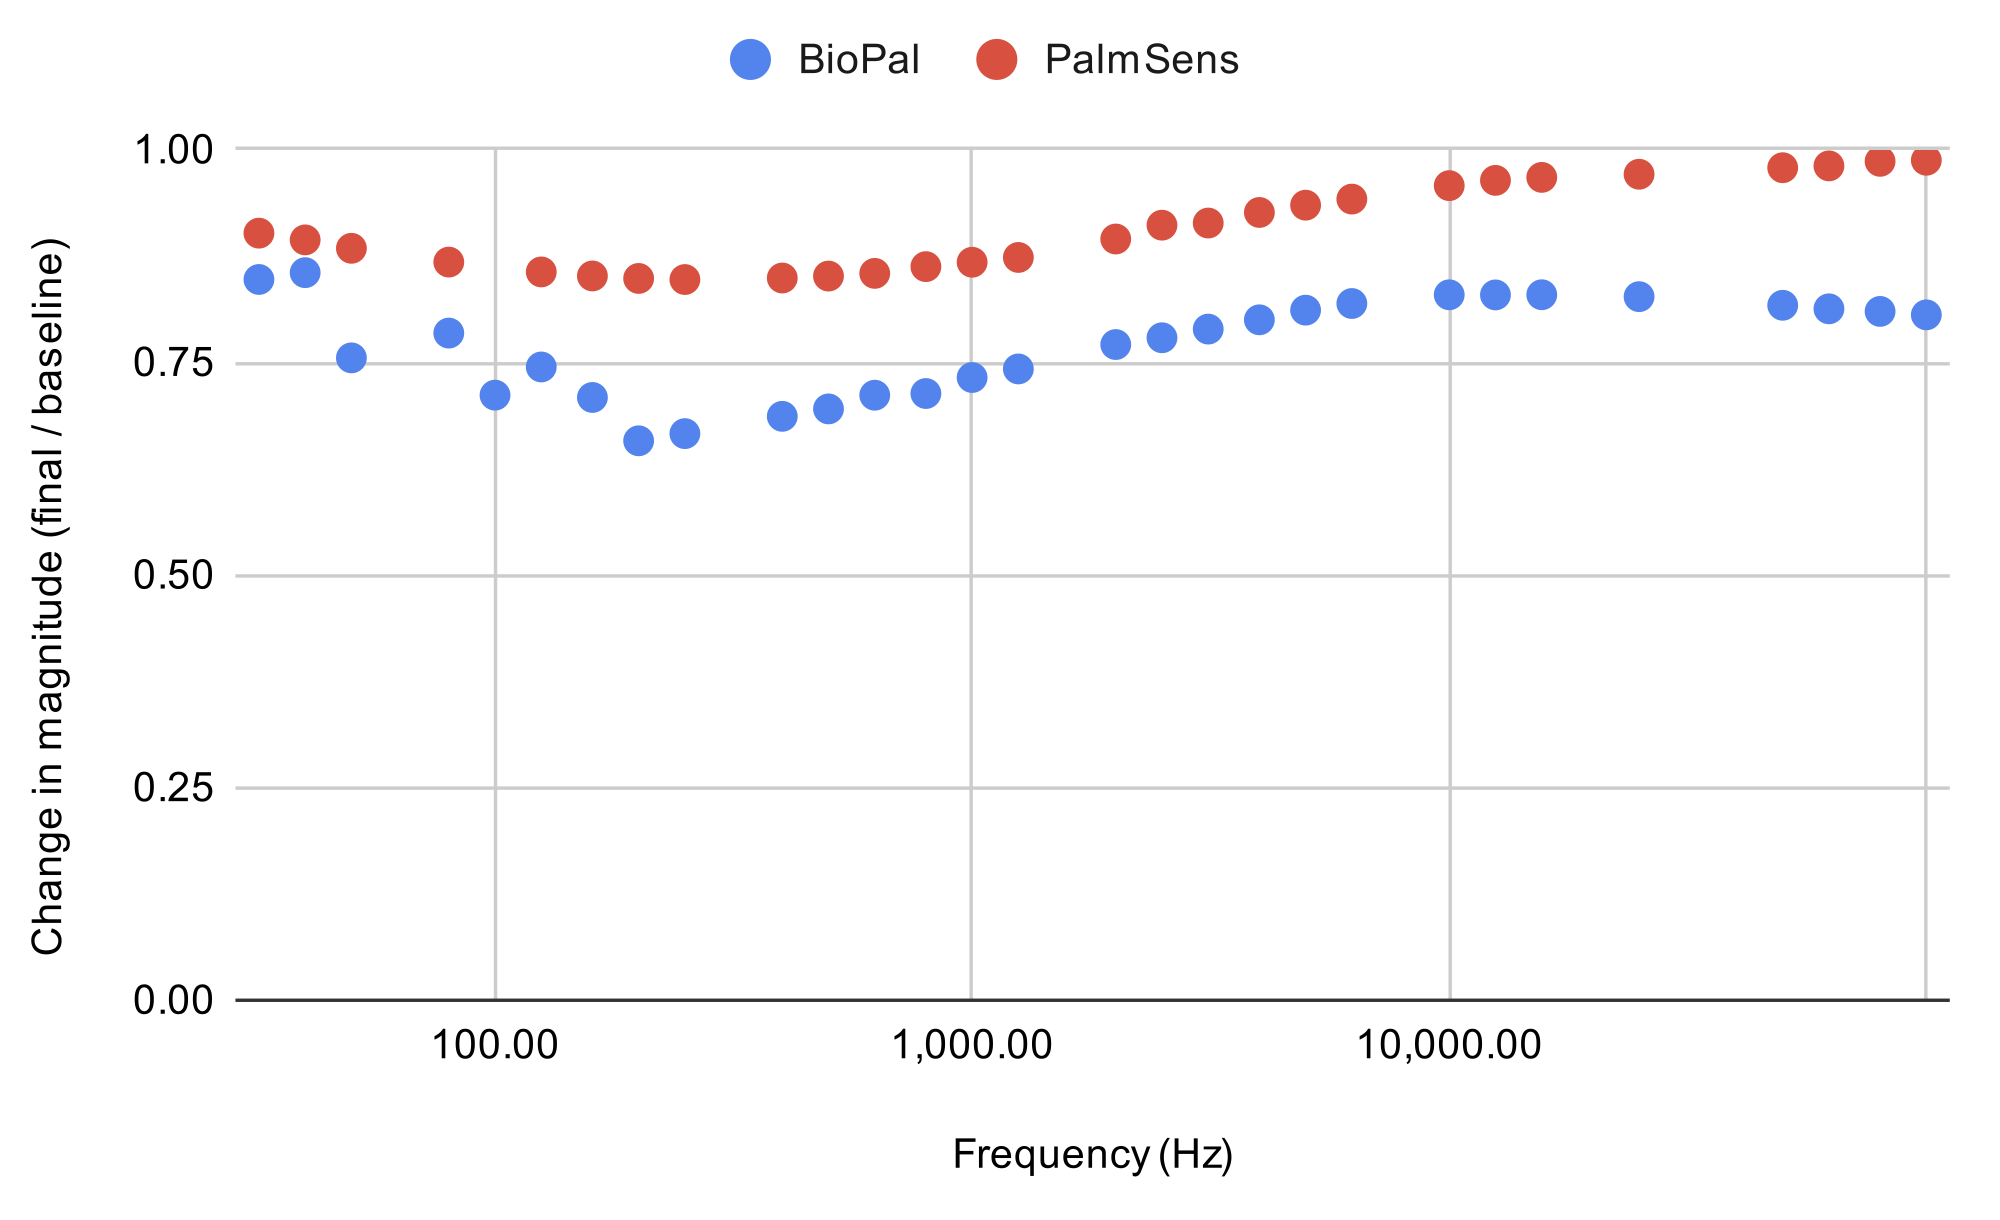
\includegraphics[width=\textwidth]{10g:100mL mag.png}   
        \caption{Change in Impedance Magnitude}
        \label{fig:10g_mag}
    \end{subfigure}
    \hfill
    \begin{subfigure}{0.48\textwidth}
        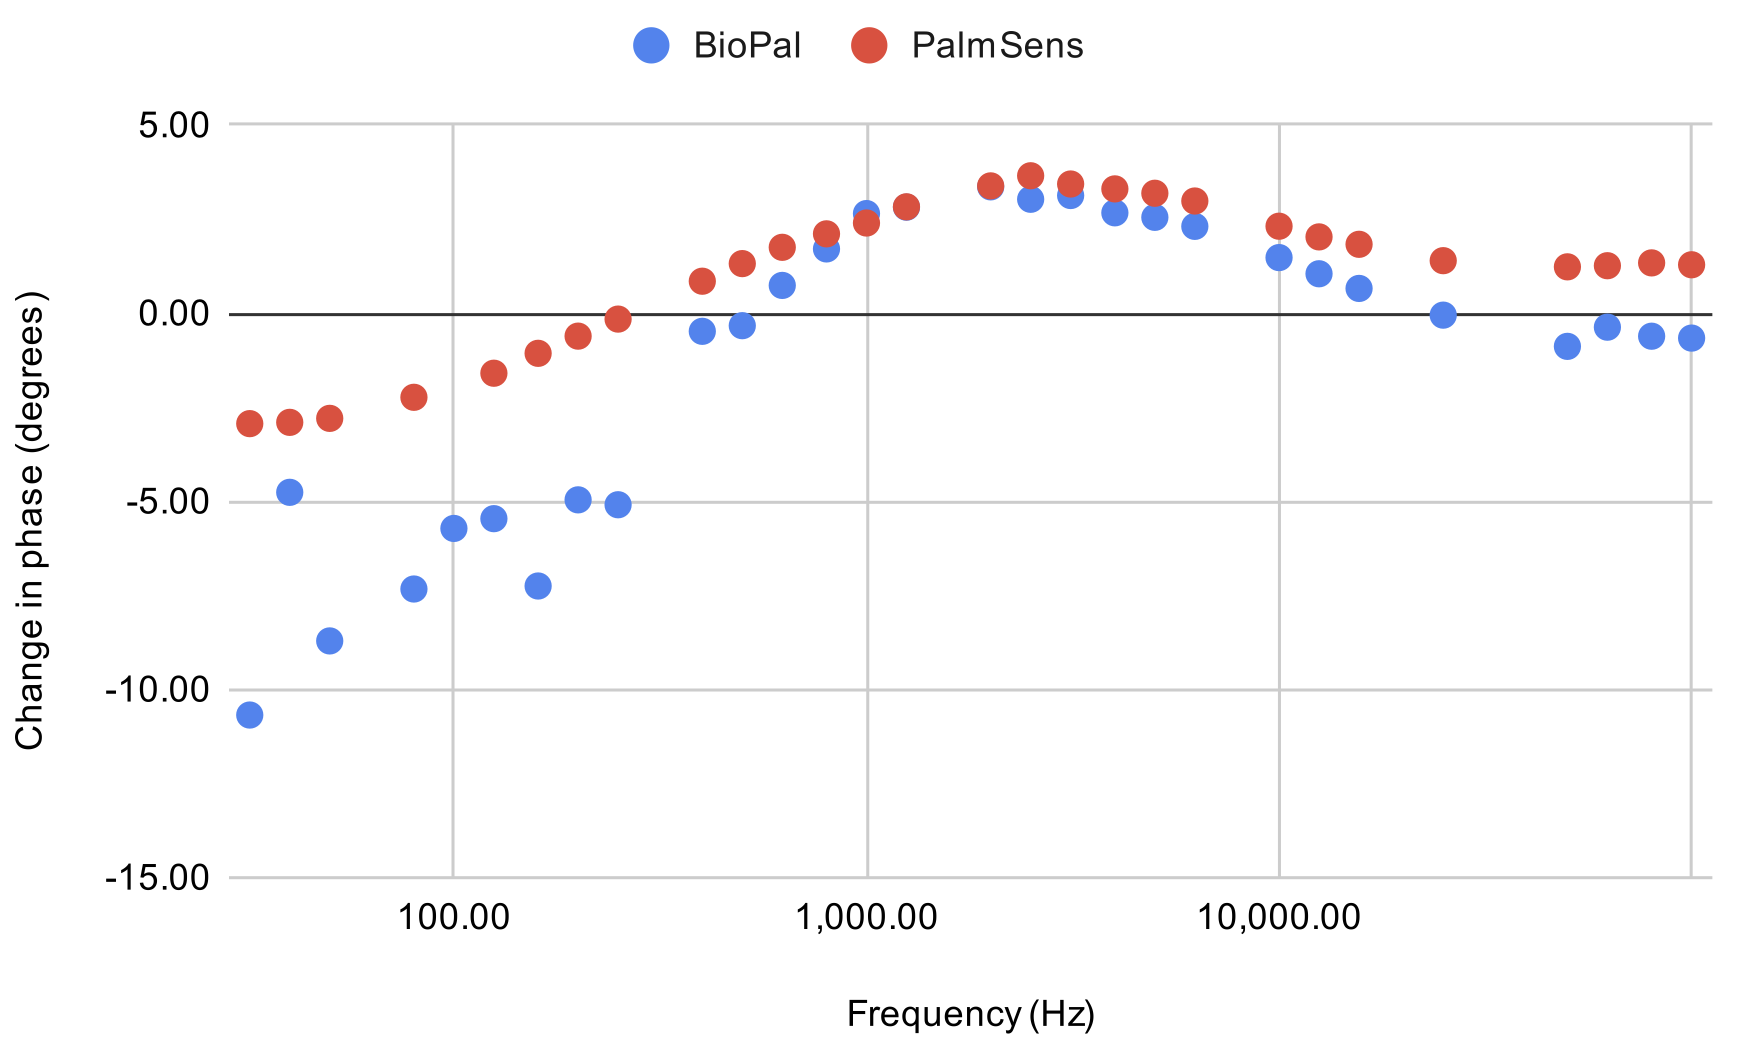
\includegraphics[width=\textwidth]{10g:100mL phase.png}
        \caption{Change in Impedance Phase}
        \label{fig:10g_phase}
    \end{subfigure}
    \caption{IDE Impedance Response to 10g/100mL BSA Binding Measured by BioPal and PalmSens4}
    \label{fig:10g_bsa_comparison}
\end{figure}

% Now the same but for the baseline vs final of each concentration for biopal and palmsens next to eachother
\begin{figure}[H]
    \centering
    \begin{subfigure}{0.48\textwidth}
        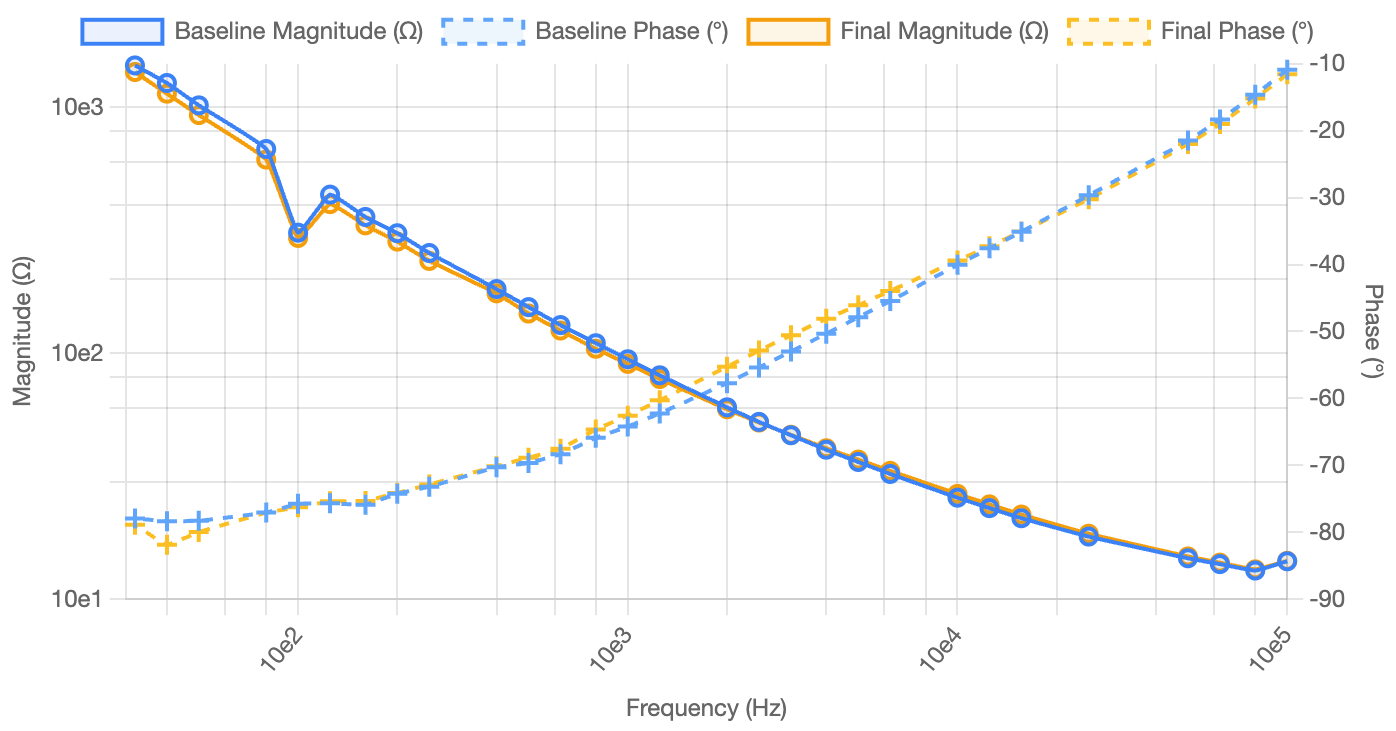
\includegraphics[width=\textwidth]{2g-100mL BioPal.png}
        \caption{BioPal: Baseline vs Post-BSA}
        \label{fig:2g_biopal}
    \end{subfigure}
    \hfill
    \begin{subfigure}{0.48\textwidth}
        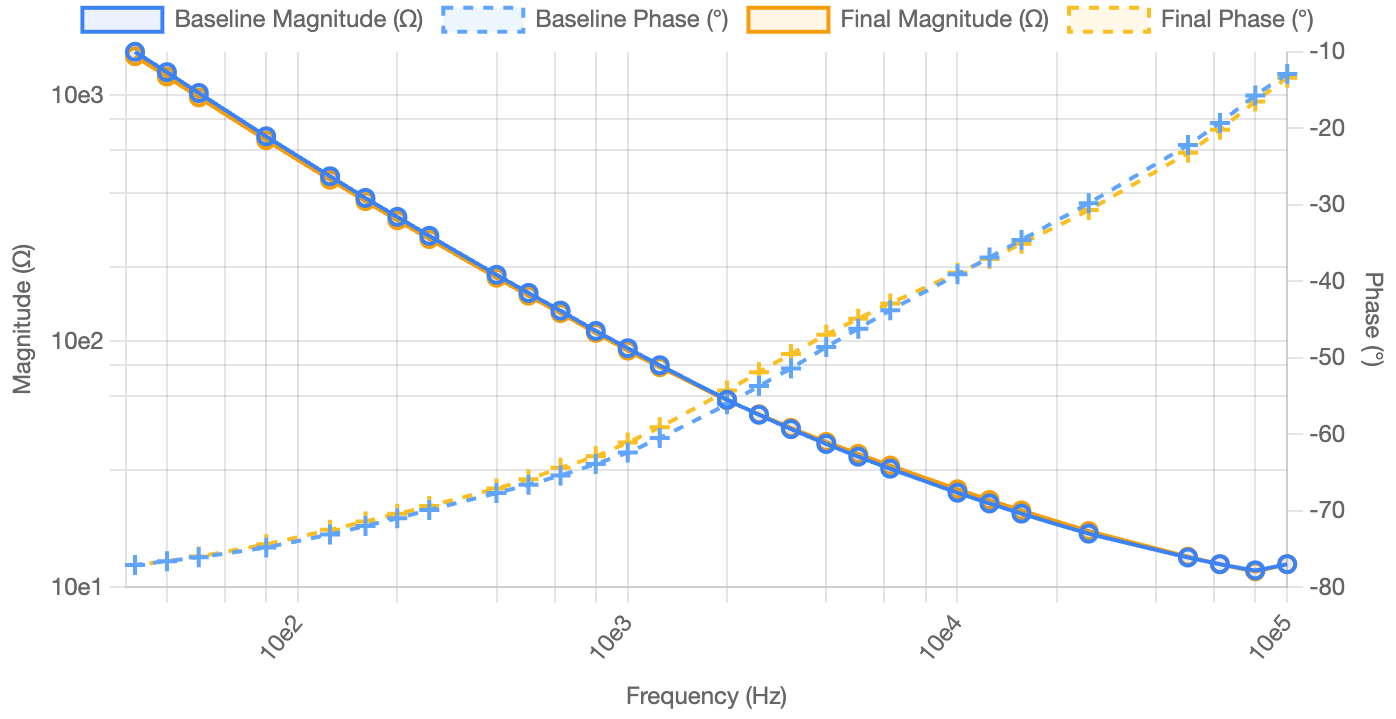
\includegraphics[width=\textwidth]{PalmSens2g.png}
        \caption{PalmSens4: Baseline vs Post-BSA}
        \label{fig:2g_palmsens}
    \end{subfigure}
    \caption{Baseline vs Final Frequency Response to 2g/100mL BSA Binding Measured by BioPal and PalmSens4}
    \label{fig:2g_bsa_comparison_final}
\end{figure}

\begin{figure}[H]
    \centering
    \begin{subfigure}{0.48\textwidth}   
        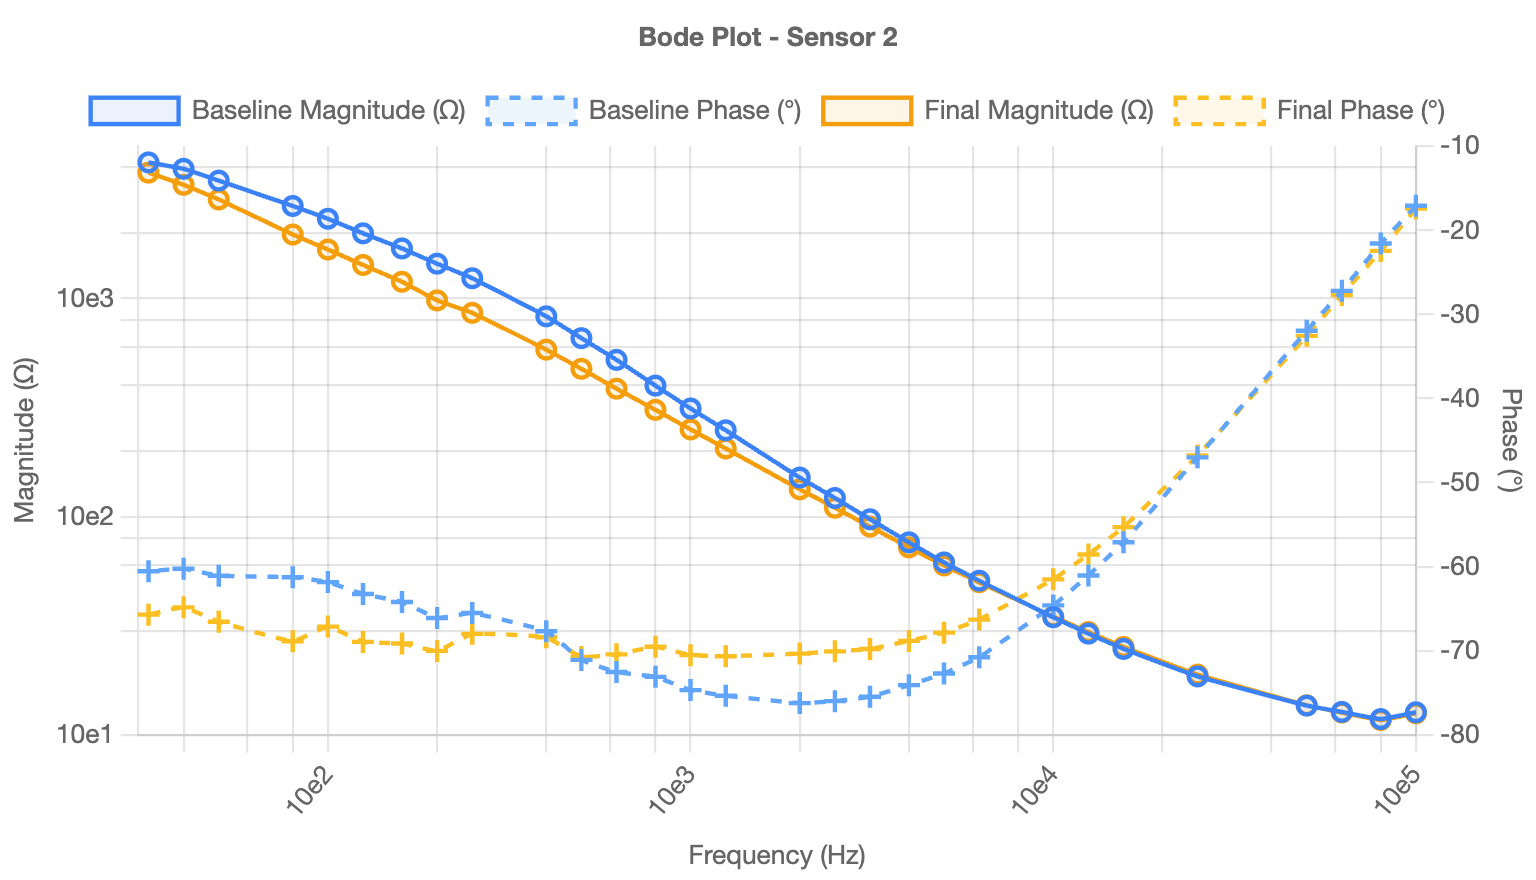
\includegraphics[width=\textwidth]{5g-100mL BioPal.png}
        \caption{BioPal: Baseline vs Post-BSA}
        \label{fig:5g_biopal}
    \end{subfigure}
    \hfill
    \begin{subfigure}{0.48\textwidth}
        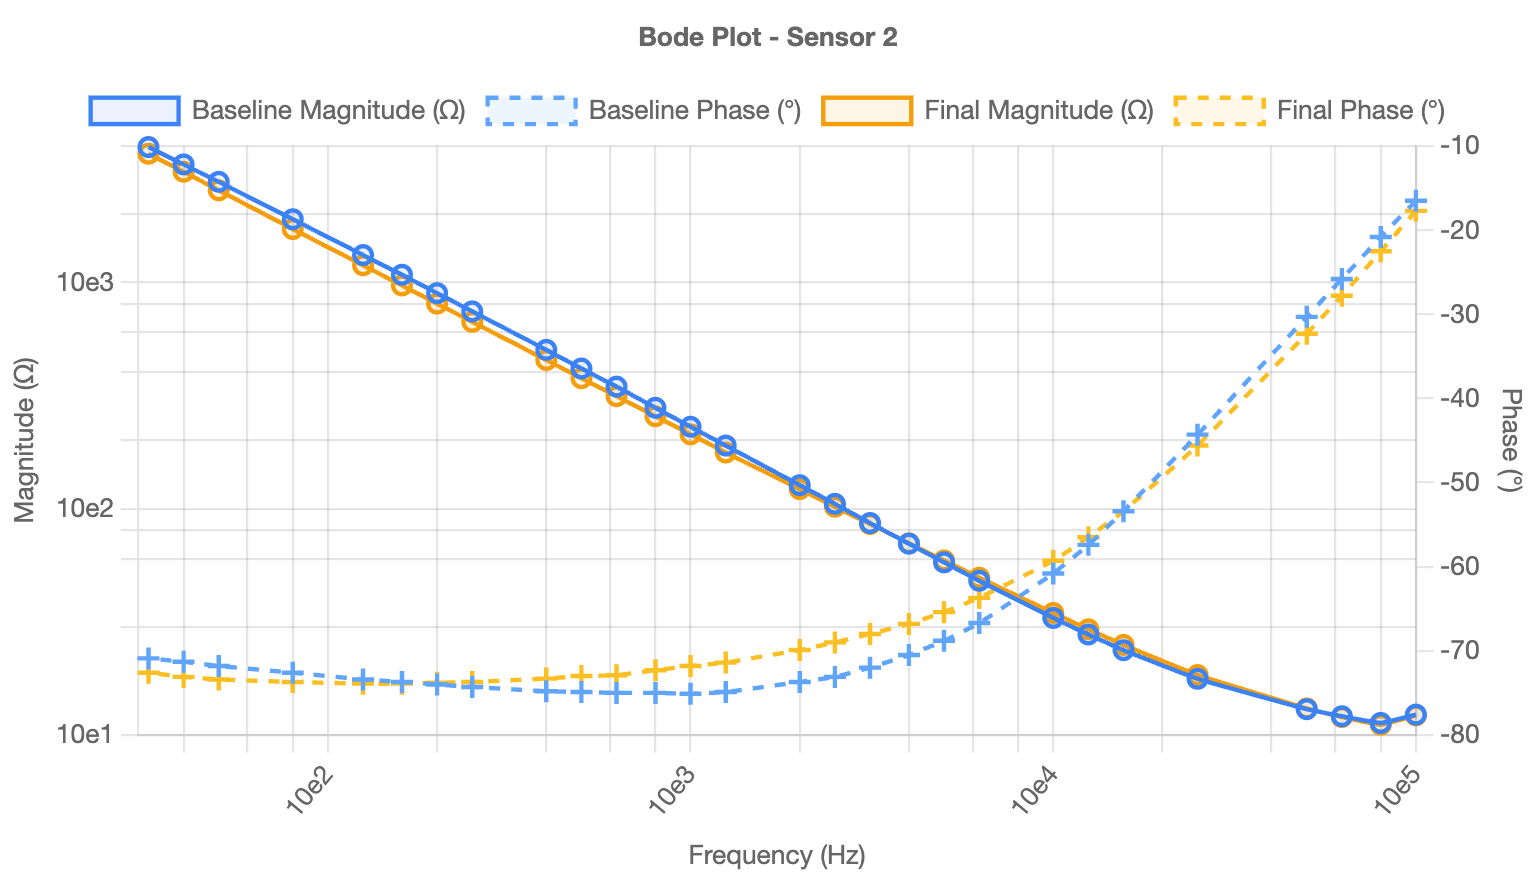
\includegraphics[width=\textwidth]{PalmSens5g.png}
        \caption{PalmSens4: Baseline vs Post-BSA}
        \label{fig:5g_palmsens}§
    \end{subfigure}
    \caption{Baseline vs Final Frequency Response to 5g/100mL BSA Binding Measured by BioPal and PalmSens4}
    \label{fig:5g_bsa_comparison_final}
\end{figure}

\begin{figure}[H]
    \centering
    \begin{subfigure}{0.48\textwidth}
        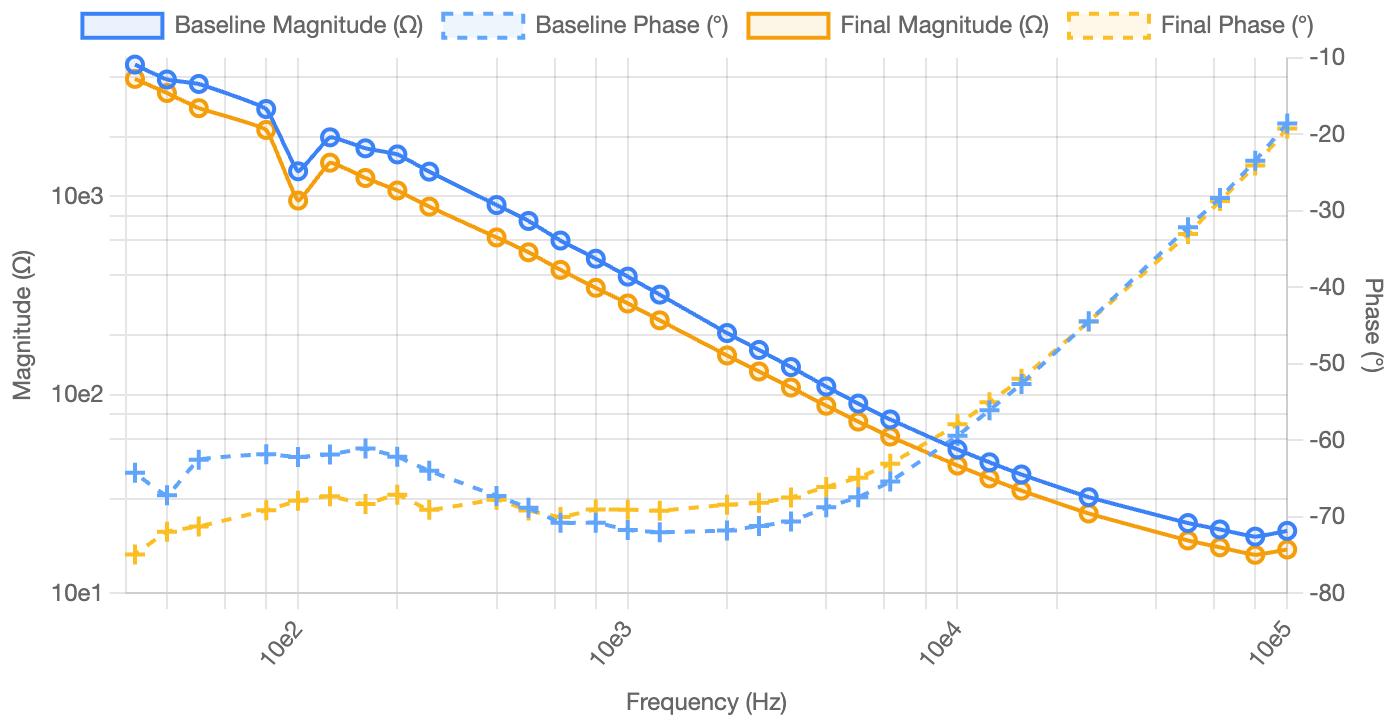
\includegraphics[width=\textwidth]{10g-100mL BioPal.png}   
        \caption{BioPal: Baseline vs Post-BSA}
        \label{fig:10g_biopal}
    \end{subfigure}
    \hfill
    \begin{subfigure}{0.48\textwidth}
        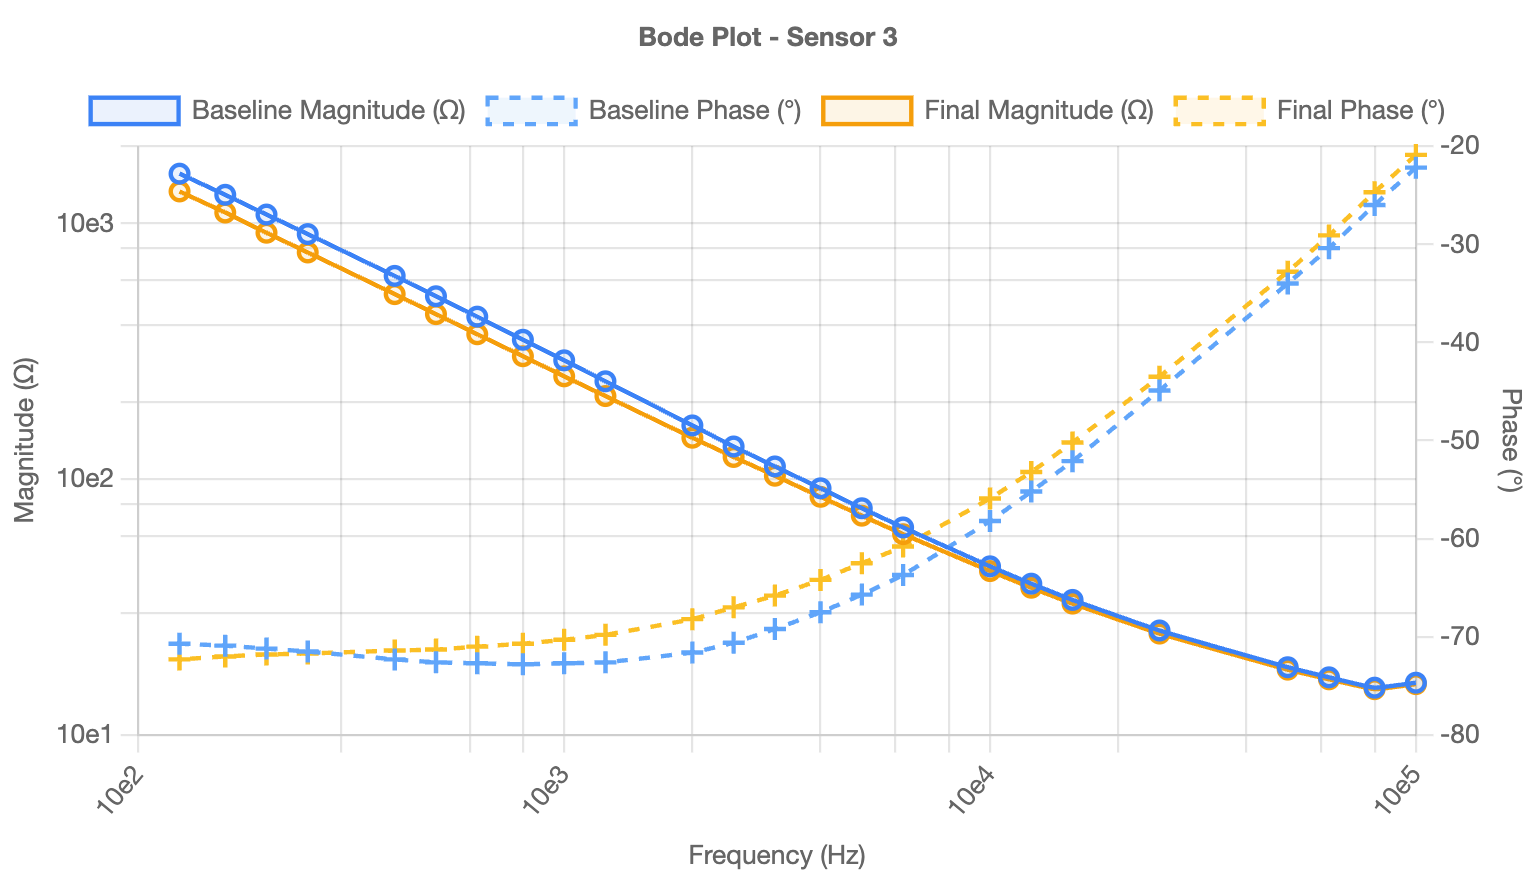
\includegraphics[width=\textwidth]{PalmSens10g.png}
        \caption{PalmSens4: Baseline vs Post-BSA}
        \label{fig:10g_palmsens}
    \end{subfigure}
    \caption{Baseline vs Final Frequency Response to 10g/100mL BSA Binding Measured by BioPal and PalmSens4}
    \label{fig:10g_bsa_comparison_final}
\end{figure}

\section{Discussion of Results}

% The BioPal's performance varied across the measurement frequency range, with distinct regions of accuracy. At very low frequencies (below \todo{X Hz}), the biosensor impedance becomes extremely high, resulting in currents in the tens of nanoamperes. At these current levels, the signal-to-noise ratio decreases substantially, making it difficult to distinguish the frequency content of interest from background noise. Consequently, measurements in this region exhibited large error margins. However, the overall trend still aligned with PalmSens4 measurements, indicating that whilst absolute accuracy was compromised, the relative changes were correctly captured.

% At slightly higher frequencies (\todo{X Hz to X Hz}), measurement accuracy improved dramatically as current levels increased and the signal-to-noise ratio became more favourable. Error margins reduced substantially, though some discrepancy from the PalmSens4 remained visible. The optimal measurement range was found to be \todo{X Hz to X Hz}, where error margins were minimal and measurements closely tracked the reference instrument. This frequency range aligns well with the region where surface characteristic changes are most prominent in EIS biosensing, making it particularly relevant for detecting analyte binding events. These are the frequencies where changes in the double-layer capacitance and charge transfer resistance due to biomolecular interactions at the electrode surface are most readily observable.

% At very high frequencies (above \todo{X Hz}), error margins increased slightly again. This can be attributed to several factors: the phase shifts in the measurement circuitry become more significant, the absence of the anti-aliasing filter allows more high-frequency noise into the system, and the parasitic capacitances and inductances in the PCB layout begin to affect measurements more noticeably.

% Despite these frequency-dependent variations in accuracy, the BioPal successfully demonstrated its core capability: detecting and quantifying impedance changes at key frequencies relevant to biosensing. The device clearly distinguished between baseline and post-BSA measurements, identifying the characteristic impedance increase associated with protein binding to the electrode surface. This validates the BioPal's applicability for quantitative biosensor measurements in point-of-care settings.

% The results demonstrate that the BioPal can provide point-of-care healthcare professionals with a low-cost, portable tool for rapid disease screening. Whilst it does not match the precision of laboratory-grade instruments like the PalmSens4 across the entire frequency spectrum, it performs well in the critical frequency ranges for biosensor applications. This enables healthcare workers to quickly screen patients and identify individuals who require further testing or specialist referral, without the need for expensive laboratory equipment or extensive technical training. The device thus fulfils its design objective of democratising biosensor-based diagnostics for resource-limited settings.

\newpage
\newpage
\label{chap:testing_and_validation}
\graphicspath{{conclusion/fig/}}

\chapter{Summary and Conclusion}
\label{chap:conclusion}
This project documents the development and testing of BioPal, a low-cost multiplexed impedance analyser aimed at point-of-care biosensing applications. The device integrates analogue frontend circuitry with embedded firmware and dual user interfaces to enable \ac{EIS} measurements on interdigitated electrodes without requiring specialised training or external equipment.

The analogue frontend implements voltage-controlled EIS across 1 Hz to 100 kHz using a 12-bit DAC for excitation, instrumentation amplifier-based voltage measurement, and transimpedance amplifier-based current measurement with programmable gain. A relay-based multiplexer enables sequential measurement of up to four \acp{IDE}. The complete system was integrated onto a custom PCB and housed in a battery-powered portable enclosure. Two user interfaces were implemented: an on-device LCD with buttons for standalone operation, and a web-based interface via Bluetooth Low Energy for enhanced usability.

The project achieved its core objectives. The analogue frontend successfully generates excitation signals and measures voltage and current responses across the target frequency range, enabling microcontroller-based EIS measurements (Objective 1). The multiplexer sequentially measures up to four IDEs (Objective 2). A complete PCB integrating all subsystems was designed and manufactured (Objective 3). Firmware implementing signal processing, FFT-based impedance calculation, and calibration correction was developed for both microcontrollers (Objective 4). Dual user interfaces enable standalone operation with qualitative risk assessment (Objective 5). The device operates from battery power with total component costs of approximately R2,000 (A full cost breakdown is shown in Table \ref{tab:cost} in Appendix \ref{appen:design}), well below the R4,500 target (Objective 6). Calibration against the PalmSens4 was completed using test cells and IDEs, with validation demonstrating sub-3\% error margins for PBS measurements and successful differentiation between varying concentrations of BSA protein binding (Objective 7).

However, several limitations constrain immediate deployment. 
\subsection{Limitations}
The inoperable LTC1069 AA filter limits accurate measurements to frequencies above 125 Hz due to aliasing artefacts, though this proved sufficient for the tested IDEs. This would be easy to replace given more time and would lead to even better accuracy and repeatability. The fixed-gain configuration improves stability but reduces flexibility for \acp{IDE} with different impedance characteristics. Validation was restricted to passive components, PBS solutions, and BSA protein. Testing with immobilised antibodies and disease biomarkers or clinical samples were outside the scope of this project. Despite these limitations, the BioPal demonstrates core measurement capabilities and a validated platform for further development toward practical \ac{POC} biosensing applications.

\subsection{Recommendations for Future Work}
Recommendations for future work towards achieving an accessible \ac{POC} biosensing system based on the BioPal platform inculde:
\begin{itemize}
    \item Enable gain settings to be configured via the user interface to accommodate \acp{IDE} with varying impedance ranges.
    \item Conduct tests using a variety of \acp{IDE} as well as immobilised antibodies and relevant disease biomarkers to evaluate real-world biosensing performance.
    \item Establish robust standardised measurement protocols to ensure consistent timing across tests.
    \item Perform user testing with healthcare workers to assess usability and workflow integration in real-world \ac{POC} settings.
\end{itemize}

These recommendations would build upon the validated BioPal platform to advance toward a practical, user-friendly impedance analyser deployed in point-of-care settings.

% Bibliography
\bibliography{mybib}

% End matter
\appendix
\chapter{Project Planning Schedule}
\makeatletter\@mkboth{}{Appendix}\makeatother
\label{appen:derivations_bigramseg}

This is an appendix.

\chapter{Outcomes Compliance}
\makeatletter\@mkboth{}{Appendix}\makeatother
\label{appen:derivations_bigramseg2}

This is another appendix.

\end{document}

